\documentclass[times, utf8, diplomski]{fer}
\usepackage{booktabs}
\usepackage{amsmath}
\usepackage{amssymb}
\usepackage{amsthm}
\usepackage{hyperref}
\usepackage{enumitem}
\usepackage{pgfplots}
\usepackage{longtable}

\pgfplotsset{width=13cm, compat=1.5}
\pgfplotsset{soldot/.style={color=black,only marks,mark=*}} \pgfplotsset{holdot/.style={color=black,fill=white,only marks,mark=*}}

\begin{document}

\renewcommand*\contentsname{Table of contents}
\newcommand\indeq{\mathrel{\overset{\makebox[0pt]{\mbox{\normalfont\tiny\sffamily ind.}}}{=}}}
% TODO: substitute theorems in the text with theorem tag
\newtheorem{proposition}{Proposition}
\newtheorem{theorem}{Theorem}
\newtheorem{definition}{Definition}

\renewcommand{\labelitemi}{$\bullet$}

\thesisnumber{2748}

\title{Option Pricing and Hedging under Jump-diffusion model}

\author{Ivan Almer}
\voditelj{Tomislav Burić}

\maketitle

% Ispis stranice s napomenom o umetanju izvornika rada. Uklonite naredbu \izvornik ako želite izbaciti tu stranicu.
% \izvornik

% Dodavanje zahvale ili prazne stranice. Ako ne želite dodati zahvalu, naredbu ostavite radi prazne stranice.
\zahvala{Thank you}

\tableofcontents

\chapter{Introduction}
% motivation
Stochastic or random process is a mathematical object which is usually defined as a collection of random variables. It can be seen as a random variable evolving over time. The weather, for example, is a stochastic process. A lot of similar examples are found in everyday life. Stochastic processes can be used to model any kind of process that, in itself, has some kind of uncertainty involved. 

Compared to a deterministic function, for which, at any time we know its value, in case of a stochastic process one cannot for sure know its value, but can maybe have an estimation or a probability of having a certain value. Although it is not ideal, it is for sure better than not knowing anything about it whatsoever. Under the assumption that processes in real world are random, but are to some degree \textit{defined}, gives us hope that, without knowing their exact future behaviour or position, we can have a good feeling of how they could move.

Stochastic processes have a very wide application in the field of finance. The main reason for that is that they can be used to model an asset price as a process where uncertainty is present. Behaviour of such processes can be observed to potentially draw some conclusions from them. 

The goal of this thesis is to utilize stochastic processes and apply them to tackle some of the problems from mathematical finance. Firstly, I will start with defining necessary mathematical and financial concepts which will be used throughout this thesis. After the foundation is set, starting with the Brownian motion, step-by-step we will arrive at the jump-diffusion process which will be used as a process of the price of an asset. We will then introduce the idea of a financial derivative, in our case an option, and we will tackle the problem of determining a fair price of the option. Lastly, we will introduce the idea of risk, how to quantify it and how to hedge the risk of our position in the asset or the option. It is my hope that, this thesis will not only provide you with a good overview of pricing and hedging of financial instruments, but also give you the understanding of such the underlying processes are useful to model the scenarios that occur every day in the market.

\chapter{Financial concepts}
% \section{General terms}
% market, trade, law of supply and demand
Let us start by defining what a market is. \textbf{Market} is a place where parties can meet to engage in an economic transaction. Usually, while only two parties are needed to make a trade, at minimum one more party is needed to introduce competition and bring balance to the market. A market in a state of \textbf{perfect competition} is characterized by a high number of active buyers and sellers. Markets vary for a number of reasons, including the types of products sold, size, location etc. One market which is of particular interest to us is the \textbf{financial market} where currencies, bonds and various types of securities are traded. They form capital and provide liquidity for businesses. Stock exchanges like New York Stock Exchange (NYSE) or Nasdaq are one type of financial markets. Other types of finincial markets include, for example bond markets and foreign exchange (FX) markets. 

As already mentioned, markets in perfect competition have a high number of participants (buyers and sellers) and market determines the prices of goods and other servides traded there. Prices are determined by \textbf{supply and demand}, where supply is created by the sellers and demand by the buyers. The law of supply and demand is a theory that explains the interaction between the sellers of a resource and the buyers for that resource. In general, if the price for a good decreases, more people are willing to buy it and less people are willing to sell. That is because the opportunity cost for the buyers decreases, as they can obtain the good at a lower price than earlier, whereas the opportunity cost for the sellers increases, as they earn less by selling the same amount of goods as before. Although it is one of the most basic economic laws, it is a part of almost all economic principles. The willingness of people to buy or sell a good determines the market equilibrium price at which the quantity of goods people are willing to sell equals the quantity of goods people are willing to buy. 

\section{Financial instruments}
% bonds, stocks, derivatives -> this will be used later
% https://www.investopedia.com/terms/f/financialinstrument.asp
In this section we will cover a few basic financial instruments. As discussed earlier, different types of markets offer different types of goods. A \textbf{bond market} (also called fixed-income markets) is a collective name attributed to all issues and trades of debt securities. Stock exchange is another type of market where, among many other things, \textbf{stocks} and \textbf{derivatives} can be traded. 

\hfill \break
A \textbf{bond} is a fixed-income financial instrument typically issued by governments or corporations in order to raise money needed to fund a certain project, for example. When a corporation (or a government) needs to borrow money, it issues bonds that include the terms of the loan, the time at which the loaned funds (bond principal) must be paid back (maturity date) and the interest payments that will be paid. They can essentially be thought of as a contract issued by the borrower promising to pay back the loan plus some interest on it at some time in the future. An interest is a premium for the person loaning the money, because by buying a bond (loaning money) the buyer takes on a risk that the issuer will not be able to pay back at maturity (risk of default). Governments are typically less likely to fail than corporations, therefore the interest paid on government bonds is genereally lower than the interest paid on corporate bonds. There are also bonds that pay additional coupons between the issuance and maturity, but they will not be of particular interest to us in the scope of this thesis.

\hfill \break
A \textbf{stock} (also called \textit{equity}) is a type of a security issued by the corporations and represents the ownership of a fraction of a company. The units of stock are called \textit{shares}. They are issued for a company to raise funds to operate their business. It is important to point out that corporations are treated as legal persons, so a shareholder does not \textit{own} a corporation, but own shares issued by the corporations and have a claim on its assets and earnings.

\hfill \break
Having explained the characteristics of bonds and stocks we arrive at securities that are not completely basic. \textbf{Derivatives} are a type of security which \textit{derives} its value from another asset (e.g. stock). There are many types of derivatives, but we will focus on the ones used in this thesis and those are options. \textbf{Option} is a contract that gives the buyer a right, but not an obligation, to buy or sell (depending on the type of the contract they hold) the underlying asset at a certain time in future. 

\hfill \break
\textbf{European options} (also called \textit{vanilla} options) are the most basic form of an option. We differentiate two different types of european options: \textit{call} and \textit{put} option. A call option gives a buyer a right to buy the underlying security at some predetermined price (strike price) at a certain time in future (maturity). In case the price of the underlying asset is greater than the strike price at the time of maturity, the buyer can buy the underlying asset at the strike price and immediately sell the asset at its market price which is now higher than the strike price, thus making a profit. However, if the price of the underlying asset is lower than the strike price at maturity, it does not make sense for the buyer to excercise the option and buy the asset at strike price, because she/he can simply buy the asset at the market price. A put option works in an opposite way, as it gives a buyer a right to sell the underlying security at the strike price at maturity. Put option expires worthless in case the price of the underlying asset is greater than the strike price as the buyer can than simply sell the security at its market price. In this case an option expires without excercising, the only loss made by the buyer is the amount paid for the option in the first place. To illustrate this very important concept of European options let us look at the following example:

\hfill \break
\noindent Suppose at time $t=0$ the price of an asset is $S_0 = 100$ and that we can buy a \textit{put} option with maturity $T$ and strike price $K=90$. The price of such option contract at time $t=0$ is $P = 5$. Let us assume that at maturity the price of the asset is $S_T = 93$. This means that the buyer will simply let the contract expire because the asset can be sold at a market price which is higher than the strike price of the \textit{put} option. If, however, the price of an asset dips below $S_0$ to value of $S_T = 80$, the buyer can buy the asset in the market for the price of $80$ and immediately sell it in the market for $K=90$ by excercising the option. Thus, making a profit of $(K-S_T) - P = (90 - 80) - 5 = 5$. 
\hfill \break
Note that in this example, the time value of money was disregarded for simplicity purposes. 

\section{Arbitrage}
% https://www.investopedia.com/terms/a/arbitrage.asp
% concept of arbitrage in continous time is too narrow so we have to use a stronger concetpt such as 'no free lunch with vanishing risk'
In finance and economics, arbitrage is the practice to take advantage of market inefficiencies to make a risk-free profit. One such inefficiency can be, for example, the difference in prices of the same asset on two different markets. In other words, an arbitrage-free market is a market where there does not exist such trade (or a set of trades) which would allow a trader with zero capital at time $t=0$ to make a positive profit at some time in future $t=T$ with positive probability. In practice, arbitrage opportunities exist, but are very hard to spot, they get almost immediately exploited and the opportunity is gone, often in the matter of seconds.\\Here are two examples to better understand this very important principle:
\subsubsection{Example 1}
Suppose that the stock XYZ is trading for \$50 on the NYSE and the same stock is trading at \$49.5 at the LSE (London Stock Exchange). The trader can then buy the stock at LSE for \$49.5 and immediately sell it at NYSE for \$50, thus realizing profit of \$0.5. 
\subsubsection{Example 2}
% TODO: do another example where P[V(T) >= 0] = 1.0 and cannot be <0
% TODO: change this to the case when S_o e^r is not between S_u and S_d
Let's see a more complex example. Suppose we have a stock XYZ with spot price $S_0 = 100$ and in one year period there are only two possibilities for the stock movement: it can go up to $S_1 = u * S_0$ where $u=1.15$, or it can go down to $S_1 = d * S_0$ where $d=0.9$. The risk-free rate in the market is constant during this one-year period and it is $r=1\%$. The probability that the stock will go up in that period is $p=0.4$. 

The inconsistency is not easy to spot here. If the market is arbitrage-free, the expected value of the future payoff should be zero. By looking more closely, and considering the time value of money one can find the following arbitrage strategy:
We decide to short-sell the stock today and put that money in the bank to be remunerated at the risk-free rate of $1\%$. After one year we take out our money from the bank and now we own the value of $(1+r)S_0 = 101$. We have to buy back the stock that we shorted one year earlier to cover this short position. There are two possible scenarios:
\hfill \break
\begin{itemize}
	\item The stock went up and our profit in that case is: $(1+r)S_0 - uS_0$ = -14
	\item The stock went down and our profit in that case is: $(1+r)S_0 - dS_0$ = 11
\end{itemize}
\hfill \break
Although at the first glance this does not look like a good deal, we have to take into account the probabilities of these events happening. More specifically, let us look at the expecte payoff at time $t=1$:

$$\mathbb{E}[\text{payoff at } t=1] = 0.4 * (-14) + 0.6 * 11 = 1$$


\newpage
\section{Fundamental theorems of asset pricing}
% bla bla about these theorems
\subsection{First fundamental theorem of asset pricing}
\begin{theorem} \label{tm:ftap1}
	A discrete market, on a discrete probability space ($\Omega$, $\mathcal{F}$, $\mathcal{P}$), is \textbf{arbitrage-free} if, and only if, there exists at least one risk neutral probability measure that is equivalent to the original probability measure, $\mathcal{P}$.
\end{theorem}

\hfill \break
This first theorem is important in that it ensures a foundamental property of market models. It will allow for some nice manipulations with discounted price processes we will mention later in this thesis.

% UNCOMMENT THE BELOW TO CONTINUE WORKING ON THE PROOF
% \subsubsection{Proof}
% % intuitive proof: https://stanford.edu/~ashlearn/RLForFinanceBook/ArbitrageCompleteness.pdf
% For illustration we will just prove the easier implication, i.e.\\\textit{Existence of Risk-neutral measure} $\Rightarrow$ \textit{Arbitrage-free}

% Suppose we have a discrete probability space ($\Omega$, $\mathcal{F}$, $\mathcal{P}$), such that $\Omega = \{\omega_1, ..., \omega_n\}$ and $\mathcal{P}: \Omega \rightarrow [0,1]$.

% \hfill \break
% A probability measure $\pi: \Omega \rightarrow [0,1]$ is said to be risk-neutral if the following holds:
% $$S_j^{(0)} = e^{-r}\sum_{i=1}^{n} \pi(\omega_i)S_j^{(i)}$$ 

\subsection{Second fundamental theorem of asset pricing}
\begin{theorem} \label{tm:ftap2}
	An arbitrage-free is said to be \textbf{complete} (every contingent claim replicable) if and only if there exists a unique risk-neutral measure equivalent to the physical one.
\end{theorem}

\hfill \break
This theorem can be reformulated in an equivalent way, that is, the market is complete if and only if there exists only one source of randomness in asset dynamic. Although this property is common in many models it is sometimes not always considered desirable or realistic. 
\chapter{Stochastic processes}
% probability and random variables
% definition of a stochastic process
% filtration
Stochastic processes have a well defined purpose in several fields, and one of those fields is finance. They seem to be the perfect choice when it comes to modelling assets' dynamics, because their \textit{randomness} is used to replicate the uncertainty of asset prices that can be observed in the market.\\

A continuous time \textbf{stochastic process} $\{X_t: t\ge 0\}$ is a collection of random variables indexed over time, often times simply $X(t)$. The probability space of these random variables is ($\Omega$, $\mathcal{F}$, $\mathbb{P}$), where $\Omega$ is the set of all possible outcomes, $\mathcal{F}$ is $\sigma$-algebra of events and $\mathbb{P}$ being the probability measure.\\
It is crucial to introduce a concept of filtration. \textbf{Filtration} $\{\mathcal{F}_t\}_{t\ge 0}$ is an increasing collection of $\sigma$-algebras, such that for every $0 \le s \le t$ the following holds: $\mathcal{F}_s \subseteq \mathcal{F}_t \subseteq \mathcal{F}$. Filtration can be thought of as \textit{"flow of information"}. More specifically, $\mathcal{F}_t$ can be considered as the information generated by all observed events up to time $t$.

\section{Brownian motion}
% Deriving Brownian motion from a random walk
The goal of this chapter is to show how Brownian motion can be derived from a random walk process. This is important to get a good understanding of what Brownian motion in fact is, as we will use it very extensively throughout the this text.

\noindent To describe the process of a \textbf{random walk} we will use a sequence of independent identically distributed (\textit{iid}) random variables $X_i$ with the following distribution:

\begin{equation}
X_i \sim \left( \begin{array}{cc} h & -h \\
					p & q \end{array} \right)
\end{equation}
Where $X_i$ describes the move of the particle in the the $i$-th step.
Let us calculate the expected value and the variance of each step:
\begin{equation}
	\begin{array}{rl}
									\mathbb{E}[X_i] &= h(p-q) \\
		Var[X_i] = \mathbb{E}[X_i^2] - \mathbb{E}[X_i]^2 &= h^2(p-q) - h^2(p-q)^2 \\
										&= h^2p + h^2q - h^2(p^2 - 2p1 + q^2)\\
										&= h^2p(1-p) + h^2q(1-q) + 2h^2pq\\
										&= 4h^2pq \\
	\end{array}
\end{equation}
Now that we have the building blocks of the random walk, let us define the state of the random walk after $n$ steps as a random variable $X(t) = \sum_{i=1}^n X_i$. Where $t$ is the length of the interval $[0,t]$. This interval is divided into $n$ equal intervals of length $\Delta t$, so we have:
\begin{equation}
	\Delta t = \frac{t}{n}
\end{equation}
We calculate the expected value and the variance of this new random variable:
\begin{equation}
	\begin{array}{rl}
		\mathbb{E}[X(t)] &= nh(p-q) \\
		Var[X(t)] &\indeq \sum_{i=1}^n Var[X_i] = 4nh^2pq \\
	\end{array}
\end{equation}
According to the Central Limit Theorem with $n \rightarrow \infty$ we know that $X(t)$ will have a normal distribution, namely:
$$ \frac{\sum_{i=1}^n X_i - nh(p-q)}{\sqrt{n}\sqrt{Var[X_i]}} = \frac{\sum_{i=1}^n X_i - nh(p-q)}{2h\sqrt{n}\sqrt{pq}} \sim \mathcal{N}(0,1) $$
$$ \Rightarrow \sum_{i=1}^n X_i - nh(p-q) \sim \mathcal{N}(0,4nh^2pq)$$
\begin{equation}
	\sum_{i=1}^n X_i \sim \mathcal{N}(nh(p-q), 4nh^2pq)
\end{equation}
we substitute $n=\frac{t}{\Delta t}$
\begin{equation}
	X(t) \sim \mathcal{N}(\mu t, \sigma^2t)
\end{equation}
\begin{equation}
	\mu := \lim_{\Delta t \to 0, h \to 0} \frac{h(p-q)}{\Delta t}
\end{equation}
\begin{equation}
	\sigma^2 := \lim_{\Delta t \to 0, h \to 0} \frac{4h^2pq}{\Delta t}
\end{equation}

Where $\mu$ is called the \textbf{drift} and $\sigma^2$ the \textbf{diffusion} of the process $X(t)$. We can have a look at the special case where $p=q=0.5$ and $h=\sqrt{t/n}=\sqrt{\Delta t}$ and it is easy to see that then $X(t)$ has the following distribution:
\begin{equation} 
	X(t) \sim \mathcal{N}(0, t)
\end{equation}	

\noindent The above mentioned process is called \textbf{Wiener process} and is often denoted by $W = \{W_t:t\ge 0\}$ where $W_t \sim \mathcal{N}(0,t)$. The formal definition is the following:

% REF: Tomas Bjork book reference
\begin{definition}[Wiener process]
A Wiener process is the process with the following properties:
\begin{enumerate}
	\item $W_0 = 0$
	\item $W_t$ is continuous in $t$
	\item $W_t$ has independent increments, i.e. for every $r < s \leq t < u$ increments $(W_u - W_t)$ and $(W_s - W_r)$ are independent random variables
	\item $W$ has Gaussian increments, i.e. for every $u,t \geq 0$: 
		\begin{equation}(W_{t+u} - W_t) \sim \mathcal{N}(0,u) \end{equation}
\end{enumerate}
\end{definition}

\section{Stochastic Integrals}
% REF: Tomas Bjork book chapter 4
As already stated in the earlier chapters, one of the objectives of this book is to study asset pricing in financial markets using stochastic processes. We want to model the price as a continuous time stochastic process and for this case the most complete and elegant theory is obtained if we use \textbf{diffusion processes} and \textbf{stochastic differential equations} as main building blocks. Although we already mentioned diffusion a couple of times, we have not really intuitively explained what it is. Loosely speaking, a stochastic process is a diffusion if its local dynamics can be approximated with the following stochastic difference equation:

\begin{equation}
	X_{t+h} - X_t = \mu(t,X_t)\Delta t + \sigma(t, X_t)\Delta W_t
\end{equation}

\noindent where $\Delta W_t$ is defined as:
\begin{equation}
	\Delta W_t = W_{t+h} - W_t
\end{equation}

\noindent If we let $h$ tend to $0$ we can write the above equation like this:
\begin{equation}
	dX_t = \mu(t,X_t)dt + \sigma(t, X_t)dW_t
\end{equation}
\noindent Which can be interpreted as a shorthand for the folowing integral equation:

\begin{equation}
	X_t = X_0 + \int_0^t \mu(s,X_s)ds + \int_0^t \sigma(s,X_s)dW_s
\end{equation}

\noindent The $ds$ integral can be viewed as a regular Riemann integral, whereas for the $dW_t$ integral we have to introduce a new concept - \textit{It\^{o} integral}.
In order to be able to construct a stochastic integral of form:
\begin{equation}
	\int_0^t g_sdW_s
\end{equation}
\noindent we have to impose some kind of integrability condition on another stochastic process $g_s$.

\begin{definition}~\\
\begin{enumerate}[label=(\roman*)]
	\item We say that the process $g_s$ belongs to the class $\mathcal{L}^2[a,b]$ if the following holds:
	\begin{itemize}
		\item $ \int_a^b\mathbb{E}[g_s^2]ds < \infty $
		\item The process $g_s$ is adapted to filtration $\mathcal{F}_t^W$
	\end{itemize}
	\item We say the process $g$ belongs to the class $\mathcal{L}^2$ if $g$ belongs to $\mathcal{L}^2[0,t]$ for every $t$
\end{enumerate}
\end{definition}

\noindent We will show how the define the stochastic integral for the case of $g_s$ which is \textbf{simple}, i.e. such $g_s$ that there exist deterministic points in time $a=t_0 < t_1 < ... < t_n = b$, such that $g$ is constant on each subinterval. To put this formally, $g_s=g_{t_k}$ where $s \in [t_k,t_{k+1})$. In that case, the stochastic integral can be defined as follows:
$$ \int_a^bg_sdW_s = \lim_{n\rightarrow\infty} \sum_{k=1}^n g_{t_k-1}(W_{t_k} - W_{t_{k-1}}) \hspace{0.5cm} \text{, where } t_k = k\frac{t}{n}$$

\noindent The process $g_s$ is evaluated in the summation on the left-hand point ($t_{k-1}$) which is known as a \textbf{non-anticipatory} integration. This is a natural choice in finance ensuring that we use no information from the fututre for our present actions.

\noindent For the case of $g_s$ which is not \textit{simple} (as described above), we would have to approximate the process $g_s$ in a certain way, but this is outside of the scope of this thesis and will not be considered because we will not encounter such integrals.

\section{Martingales}
% REF: Tomas Bjork book
Theory of stochastic integration is closely related to the theory of martingales. Moreover, it is a foundation of the modern theory of financial derivatives. It would be unreasonable to not mention this topic, because of its extreme importance in the field. In discrete time, we say a stochastic process is a \textbf{martingale} if for any time $n$ the following properties hold:

\begin{center}
	\begin{itemize}
		\item $\mathbb{E}[|X_n|] < \infty$
		\item $\mathbb{E}[X_n | X_0, ..., X_{n-1}] = X_{n-1}$
	\end{itemize}
\end{center}

Where the first condition is more of a \textit{technical} condition and the second one is the most important one. The second condition states that if at any time $t=n$ we look at the expected value of the process at any time $t>n$, it is equal to the value of the process at time $t=n$. A process that is a martingale can be viewed as a model of a fair game.

\noindent In order to extend the definition of a martingale to a continuous case, let us first consider a concept of filtration ${\mathcal{F}}_{t \ge 0}$, that we have already mentioned earlier. As before, a filtration can be thought of as a \textit{flow of information} and $\mathcal{F}_t$ as the information generated by all observed events up to time $t$. For any random variable $X$ let the symbol
$$\mathbb{E}[X|\mathcal{F}_t]$$
represent the \textit{"expected value of $X$ given the information available up to time $t$"}. It is important to note here that for a fixed $t$, the object $\mathbb{E}[X|\mathcal{F}_t]$ is a random variable. Let, for example, a filtration be generated by the process $Y$, then the information available up to time $t$ will, of course, be dependent on the behaviour of the process $Y$ in the time interval $[0,t]$. Before defining a continous time martingale, let us first consider the following proposition:

\begin{itemize}
	\item \textit{If $Y$ and $Z$ are random variables, and $Z$ is $\mathcal{F}_t$-measurable (known at time $t$), then} $$\mathbb{E}[Z\cdot Y|\mathcal{F}_t] = Z \cdot \mathbb{E}[Y|\mathcal{F}_t]$$
	\item \textit{If $Y$ is a random variable and $s<t$, then} $$\mathbb{E}[\mathbb{E}[Y|\mathcal{F}_t]|\mathcal{F}_s] = \mathbb{E}[Y|\mathcal{F}_s]$$
\end{itemize}

\begin{definition}
A stochastic process $X$ is an $(\mathcal{F}_t)$-martingale if the following conditions hold:
\begin{itemize}
	\item $X$ is adapted to filtration $\{\mathcal{F}_t\}_{t\geq 0}$
	\item For all $t$ we have $$\mathbb{E}[|X_t|] < \infty$$
	\item For all $s$ and $t$, where $s\leq t$ we have $$\mathbb{E}[X_t|\mathcal{F}_s] = X_s$$
\end{itemize}
\end{definition}

The first condition above is a condition saying that the process $X_t$ is observable (known) at time $t$. The second one, like in discrete case, is just a technical condition. Also like in discrete case, the third condition is the important one, which states that the expected future value of the $X$, given the information available today, is equal to today's observed value of $X$. In other words, a martingale has an absence of drift.

\section{Stochastic Calculus and It\^{o}'s Lemma}
% LAST ANSWER HERE: https://math.stackexchange.com/questions/2686925/some-questions-on-the-details-of-an-integration-of-brownian-motion-against-itsel
When talking about stochastic processes, one can see that they are different than the usual functions. If we look at a infinitesimally small time interval $\Delta t$ and observe the function behaviourin that time interval, the function is a straight line. This is unfortunately not the case with the stochastic processes, where even if we \textit{zoom-in} on the trajectory, the trajectory is not smooth. Therefore, a japanese mathematician Kiyoshi It\^{o} started and created the field of \textbf{stochastic calculus} which is able to operate on stochastic processes. 

We come to the very important theorem in the field of stochastic calculus and that is \textbf{It\^{o}'s lemma}.

\begin{theorem}[It\^{o}'s Lemma]
Assume that the process $X$ has a stochastic differential given by $$dX_t = \mu_t X_t dt + \sigma_t X_t dW_t$$ where $\mu$ and $\sigma$ are adapted processes, and let $f$ be a $C^{1,2}$-function. Define the process $Z$ by $Z(t) = f(t,X_t)$. Then $Z$ has a stochastic differential given by 
$$df(t, X_t) = \left(\frac{\partial f}{\partial t} + \mu_t X_t \frac{\partial f}{\partial x}+\frac{1}{2}\sigma_t^2 X_t^2 \frac{\partial^2f}{\partial x^2}\right)dt + \sigma X_t \frac{\partial f}{\partial x}dW_t$$
\end{theorem}
\noindent A proof of this theorem is outside the scope of this thesis and it is rather cumbersome. The power and importance of this theorem is that we can define the differential of a function of a stochastic process. This will prove to be an indispensible tool when we will be pricing an option, as the price of the option depends on the price of an asset, which means it is a function of the asset price. 

\noindent We also introduce an alternative, more general, form of It\^{o}'s lemma which we will use in the following section to obtain an expression for the process governed by the geometric Brownian motion:
\begin{equation} \label{eqn:ito_general}
	df = \frac{\partial f}{\partial t}dt + \frac{\partial f}{\partial x}dX_t + \frac{1}{2}\frac{\partial^2 f}{\partial x^2}(dX_t)^2
\end{equation}

\subsection{Geometric Brownian motion} \label{section_gbm}
% https://medium.com/the-quant-journey/a-gentle-introduction-to-geometric-brownian-motion-in-finance-68c37ba6f828
Let us now show how to apply It\^{o}'s formula for the case of \textit{geometric Brownian motion}. Before we start, it is crucial to first describe what kind of process that is. 

\begin{definition}
A process $X$ is said to be a \textbf{geometric Brownian motion} if it satisfies the following stochastic differential equation:

\begin{equation}
	dX_t = \mu_t X_t dt + \sigma_t X_t dW_t
\end{equation}

\end{definition}

\noindent where $\mu_t$ and $\sigma_t$ are \textit{drift} and \textit{diffusion} (respectively) of the process $X$. $W_t$ is the basic Brownian motion, that is, $W_t \sim \mathcal{N}(0,t)$. Let us now consider a function $f(t,X_t) = \ln(X_t)$ which, of course, yields another stochastic process. We will employ an alternative form of It\^{o}'s lemma found in the equation \ref{eqn:ito_general}. If we expand the $(dX_t)^2$ we get: 
\begin{equation}
	(dX_t)^2 = (\mu_t X_t dt + \sigma_t X_t dW_t)^2 = \mu_t^2 X_t^2 (dt)^2 + 2\mu_t\sigma_tX_t^2dtdW_t + \sigma_t^2X_t^2(dW_t)^2
\end{equation}
where we use the formal multiplication table: 

\begin{equation} 
	\left\{ \begin{array}{c} (dt)^2 = 0, \\ dt\cdot dW_t = 0, \\ (dW_t)^2 = dt \end{array} \right. 
\end{equation} so we have: 
\begin{equation}
	(dX_t)^2 = \sigma_t^2X_t^2dt
\end{equation}
Before we apply the It\^{o}'s formula to this problem, let us first calculate the partial derivatives that appear in the formula. 
\begin{equation}
	\frac{\partial \ln(X_t)}{\partial t} = 0 \hspace{0.25cm} ; \hspace{0.25cm} \frac{\partial \ln(X_t)}{\partial x} = \frac{1}{x} \hspace{0.25cm} ; \hspace{0.25cm} \frac{\partial^2 \ln(X_t)}{\partial x^2} = -\frac{1}{x^2}
\end{equation}

Now we are finally ready to apply the formula. We will step by step derive the formula for $X_t$:
\begin{equation*}
	df = 0\cdot dt + \frac{1}{X_t}dX_t - \frac{1}{2} \frac{1}{X_t^2}(dX_t)^2 
\end{equation*}
\begin{equation*}
	df = \frac{1}{X_t} (\mu_t X_t dt + \sigma_t X_t dW_t) - \frac{1}{2}\frac{1}{X_t^2}\sigma_t^2 X_t^2 dt
\end{equation*}
\begin{equation}
	df = (\mu_t - \frac{1}{2}\sigma_t^2)dt + \sigma_t dW_t
\end{equation}
and if we integrate it over the time interval $[0,t]$ we get
\begin{equation}
	\int_0^t df(s) = \int_0^t (\mu_s - \frac{1}{2}\sigma_s^2) ds + \int_0^t \sigma_s dW_s
\end{equation}
For simplicity purposes, let us assume that $\mu$ and $\sigma$ are constants. Then they can come outside of the integral and the resulting formula is
\begin{equation}
	\ln(X_t) - \ln(X) = (\mu-\frac{1}{2}\sigma^2)t + \sigma (W_t - W_0)
\end{equation}
Remembering that the $W_0 = 0$ we get the following result:
\begin{equation*}
	\ln\frac{X_t}{X_0} = (\mu-\frac{1}{2}\sigma^2)t + \sigma W_t
\end{equation*}
\begin{equation} \label{eqn_gbm}
	X_t = X_0\exp\left\{ (\mu-\frac{1}{2}\sigma^2)t + \sigma W_t \right\}
\end{equation}

This model is in finance also known as \textbf{log-normal asset return model}, because we are using logarithmic prices. It is important to note that this model only has \textbf{positive values} of stock prices, which is in that sense in line with the real world, where stock prices can not become negative. 

\vspace{1cm}
\begin{figure}[ht]
\centering
\begin{tikzpicture}
\begin{axis}[
    title={Geometric Brownian motion ($\mu$=0.05, $\sigma$ = 0.4)},
    xlabel={t},
    ylabel={Price},
    xmin=0, xmax=1,
    ymin=30, ymax=210,
    ymajorgrids=true,
    grid style=dashed,
]
\addplot[color=orange] table {data/gbm1.dat};
\addplot[color=magenta] table {data/gbm2.dat};
\addplot[color=teal] table {data/gbm3.dat};
\addplot[color=olive] table {data/gbm4.dat};
\end{axis}
\end{tikzpicture}
\caption{Geometric Brownian motion paths for parameters $\mu$=0.05 and $\sigma$ = 0.4}
\label{fig:gbm_paths}
\end{figure}

\chapter{Pricing an asset}
The famous Black-Scholes model assumes that the price of the asset follows the geometric Brownian motion we have just covered. Geometric Brownian motion satisfies a local Markov property, that is, the change in the value of the process in a very small amount of time can only be marginal. The distribution of returns of the geometric Brownian motion is not completely comparable to the real world scenario. To be more specific, in real world from time to time there is a shock hitting the market and the prices move rapidly in some direction. Such movements are called jumps. The problem with the geometric Brownian motion is that it does not allow for such events to happen, therefore yielding a return distribution with thinner tails than what would be the case in real markets. It is of interest to us to try and model such events. The idea was previously introduced in \cite{merton_option_1976}. In this section we will describe the building blocks of such process and arrive to the dynamics which have to be satisfied for the process to be a Jump-diffusion process.

	\section{Poisson process}
	Poisson process and exponential distribution are very closely linked so let us have a look at exponential distribution first. Poisson process has some convenient mathematical properties, which has led to it being used as a mathematical model for seemingly random processes in various disciplines, including, of course, economics. It is named after French mathematician Simeon Denis Poisson despite the fact that he has never studied this process. The reason why it is called a Poisson process is that if a collection of points in some space forms a Poisson process than the number of those points in a finite size region is a random variable with a Poisson distribution. This will be step by step explained in next sections.
		\subsection{Exponential distribution}
		As mentioned earlier, exponential distribution is very closely linked to the Poisson process as the time between events in Poisson process has exponential distribution. It is a continuous analogue of the geometric distribution.
			\begin{definition}[Exponential distribution]
			\label{exponential}
			We say that a random variable $X$ is exponentially distributed if its probability density function (PDF) is:
			\begin{equation}
				f(x) = \left\{ \begin{array}{lc} \lambda e^{-\lambda x} &, x \geq 0 \\
												0 &, x < 0 \end{array}\right.
			\end{equation}

			\noindent where $\lambda > 0$ is the parameter of the distribution, often called the rate parameter. The notation to indicate that a random variable is exponentially distributed is $$X \sim \varepsilon(\lambda)$$
			\end{definition}

			% REF: memorylessness -> https://en.wikipedia.org/wiki/Memorylessness
			\noindent The expected value of a random variable $X$ which is exponentially distributed is \begin{equation} \mathbb{E}[X] = \frac{1}{\lambda} \end{equation} The most famous property of the exponential distribution is memorylessness. \textbf{Memorylessness} is a property of certain probability distributions which refers to the fact that the waiting time until the occurrence of a certain event does not depend on how mych time has already elapsed. Memorylessness of an exponential distribution is formally expressed as: \begin{equation} P(X > t + s | X>s) = e^{-\lambda t} = P(X > t) \end{equation} If $X$ is a random variable modelling a waiting time, this would mean that the probability that we wait more than $t+s$ if we already know that at least $s$ time has elapsed, is the same as the probability that we will wait more than $t$. 
		\subsection{Defining a Poisson process}
		A \textbf{Poisson process} registers the occurrences of the certain event in a finite time interval. It notes the number of occurrences as well as times when the event happened. 
		\begin{definition}[Poisson process]
			Poisson process $(N_t, t \geq 0)$ is given by the following conditions:
			\begin{enumerate}
				\item $N_0 = 0$
				\item $N$ has independent increments
				\item Random variable $N(s,t) = N_t - N_s$ where $0 \leq s \leq t$, has a Poisson distribution with parameter $\lambda (t-s)$, that is, 
				\begin{equation} P(N_t - N_s = n) = e^{-\lambda(t-s)}\frac{[\lambda(t-s)]^n}{n!} \end{equation}
			\end{enumerate}
		\end{definition}

		% TODO: automate this part to be generated by the python script
		\begin{figure}[ht]
		\centering
		\begin{tikzpicture}
		\begin{axis}[
		    % title={Poisson process with $\lambda = 4$},
		    xlabel={t},
		    xmin=0, xmax=1,
		    ymin=0, ymax=5,
		    ytick={1,2,3,4,5},
		    ymajorgrids=true,
		    grid style=dashed,
		]
		\addplot[semithick, domain=0:0.08372,black] {0};
		\addplot[semithick, domain=0.08372:0.49,black] {1};
		\addplot[semithick, domain=0.49:0.87997,black] {2};
		\addplot[semithick, domain=0.87997:0.949862,black] {3};
		\addplot[semithick, domain=0.949862:1.0,black] {4};
		\draw[dotted] (axis cs:0.08372,0) -- (axis cs:0.08372,1);
		\draw[dotted] (axis cs:0.49,1) -- (axis cs:0.49,2);
		\draw[dotted] (axis cs:0.87997,2) -- (axis cs:0.87997,3);
		\draw[dotted] (axis cs:0.949862,3) -- (axis cs:0.949862,4);
		\draw[dotted] (axis cs:6,6) -- (axis cs:6,-5);
		\addplot[holdot] coordinates{(0.08372,0)(0.49,1)(0.87997,2)(0.949862,3)};
		\addplot[soldot] coordinates{(0,0)(0.08372,1)(0.49,2)(0.87997,3)(0.949862,4)};
		\end{axis}
		\end{tikzpicture}
		\caption{Poisson process path with deterministic increment of $1$ and parameter $\lambda = 4$}
	 	\label{fig:poisson_process}
		\end{figure}

		% REF: Derivative security pricing book pg. 253
		\noindent There is an alternative definition of a Poisson process which we will use when we will be defining a jump-diffusion process. As we already mentioned before, Poisson process registers occurrences of a certain event on a \textit{finite time interval}. If we let that interval to become very small and denote it by $h$, we denote the probabilities of the number occurrences by: 
		\begin{equation}
			\begin{array}{rcl}
				P(N(h) \geq 2) &\mbox{=}& o(h) \\
				P(N(h) = 1) &\mbox{=}& \lambda h \\
				P(N(h) = 0) &\mbox{=}& 1 - \lambda h + o(h)
			\end{array}
		\end{equation}
		Where $o(h)$ is infinitesimally small amount, that is, some function with with the property: \begin{equation} \lim_{h \to 0} \frac{o(h)}{h} = 0 \end{equation} Then we can let $dN$ denote an increment in the Poisson process on an infinitesimally small time interval $dt$. 
		\begin{equation} 
			dN = \left\{  \begin{array}{lcl} 1 & \mbox{with probability} & \lambda dt \\
																	0 & \mbox{with probability} & (1 - \lambda dt) \end{array} \right.
		\end{equation}
	
	\section{Pure Jump process}
		\subsection{Definition}
		Now that the Poisson process has been explained, it will be easy to understand the Jump process. Like we stated earlier, the Poisson process registers occurrences of certain events. When talking about a jump process those events that occur will be the jumps. On each such event the value of our Jump process will be increased by a ceratin value (it will \textit{"jump"}). The initial value of the Jump process is $J(0) = 0$. The size of the $i$-th jump will be a random variable $U_i$ independant of the Poisson process, that is, $N(t) \bot U_i$ , $\forall i$. All $U_i$ are independent and identically distributed random variables (\textit{iid}).

		% REF: DSP pg. 255
		\begin{definition}
			We define a Jump process as 
			\begin{equation}
				J(t) = \sum_{i=1}^{N(t)} U_i
			\end{equation}
			assuming $J(0) = 0$. The Jump process is right-continuous.
		\end{definition}

		We will use $\mathbb{Q}_j$ and $\mathbb{Q}_u$ to indicate the probability measure governing the jump arrival times and the probability measure governing the jump sizes, respectively. We assume independence of the mentioned probability measures. Let us now have a look at the expected value of the Jump process we have just defined:

		\begin{equation} \label{eqn_e_jump} % \ref{eqn_e_jump}
		\mathbb{E}[J(t)] = \mathbb{E}^{\mathbb{Q}_j}\mathbb{E}^{\mathbb{Q}_u} \sum_{i=1}^{N(t)} U_i
		\end{equation}

		\noindent When performing the calculation we have to have in mind that $\mathbb{E}^{\mathbb{Q}_u}[U_i] = k$.

		\begin{equation}
		\begin{split}
			\mathbb{E}[J(t)] &= \sum_{n=0}^{\infty}\mathbb{E}^{\mathbb{Q}_u} \left[ \sum_{i=1}^{n} U_i \right] P(N(t)=n) = \sum_{n=0}^{\infty}\sum_{i=1}^{n} \mathbb{E}^{\mathbb{Q}_u}\left[U_i\right] P(N(t)=n) \\
			&= \sum_{n=0}^{\infty} nk\frac{(\lambda t)^n}{n!}e^{-\lambda t} = \sum_{n=1}^{\infty} nk\frac{(\lambda t)^n}{n!}e^{-\lambda t} \\
			&= ke^{-\lambda t}\lambda t\sum_{n=1}^{\infty}\frac{(\lambda t)^{n-1}}{(n-1)!} = k\lambda te^{-\lambda t}\sum_{n=1}^{\infty}\frac{(\lambda t)^n}{n!} \\
			&= k\lambda t
		\end{split}
		\end{equation}

		% \vspace{1cm}
		\begin{figure}
		\centering
		\begin{tikzpicture}
		\begin{axis}[
		    % title={Pure Jump Process with $\lambda$ = 6 and jump size $U \sim \mathcal{N}(\mu=0,\sigma^2=0.04)$},
		    xlabel={t},
		    % ylabel={Price},
		    xmin=0, xmax=1,
		    % ymin=30, ymax=210,
		    ymajorgrids=true,
		    grid style=dashed,
		]
		\addplot[semithick, color=magenta] table {data/jump_process_path1.dat};
		\addplot[semithick, color=teal] table {data/jump_process_path2.dat};
		\addplot[semithick, color=olive] table {data/jump_process_path3.dat};
		\end{axis}
		\end{tikzpicture}
		\caption{Pure Jump Process with $\lambda$ = 6 and jump size $U \sim \mathcal{N}(\mu=0,\sigma^2=0.04)$}
		\label{fig:pure_jump_process}
		\end{figure}

		\noindent As we can see the the expected value of the Jump process at time $t$ is different than $0$ which will subsequently lead to the conclusion that the process $J(t)$ is not a martingale. Sometimes it is useful to work with a Jump process which, in turn, is a martingale. Such process is called a \textbf{compensated Jump process}. 
		
		\begin{proposition} Let us denote a compensated Jump process with $\tilde{J}(t)$ and let it be defined by:
			\begin{equation}
			\tilde{J}(t) := J(t) - k\lambda t
			\end{equation}
			Such a process is a martingale.
		\end{proposition}
		\begin{proof}
			Let us assume we that we have $0 \leq s \leq t$ and we determine the expected value of the $\tilde{J}(t)$ given that we have information up to time $s$:
			\begin{align*}
				\mathbb{E}[\tilde{J}(t)|\mathcal{F}_s] &= \mathbb{E}[\tilde{J}(t) + \tilde{J}(s) - \tilde{J}(s)|\mathcal{F}_s] \\
				&= \mathbb{E}[\tilde{J}(t) - \tilde{J}(s)|\mathcal{F}_s] + \mathbb{E}[\tilde{J}(s)|\mathcal{F}_s] \\
				&= \mathbb{E}[\tilde{J}(t - s)] + \tilde{J}(s) \hspace{3cm} \mbox{\textit{(independent increments)}} \\
				&= \mathbb{E}[J(t - s) - k\lambda (t-s)] + \tilde{J}(s)\\
				&= k\lambda (t-s) - k\lambda (t-s) + \tilde{J}(s) \\
				&= \tilde{J}(s)
			\end{align*}
		\end{proof}

	Before we continue further and comobine the knowledge we have on geometric Brownian motion and Jump processes to obtain a Jump-diffusion process, let us first denote with $d\tilde{J}$ the change in the compensated Jump process in an infinitesimally small time interval $dt$:
	\begin{equation}
		d\tilde{J} = \left\{  \begin{array}{lcl} U_i - k\lambda dt& \mbox{with probability} & \lambda dt \\
																	- k\lambda dt & \mbox{with probability} & (1 - \lambda dt) \end{array} \right.
	\end{equation}

	\section{Jump-diffusion process}
	This has led us to the final part where we will obtain the final process of our asset price. This process will be the combination of the geometric Brownian motion and a (compensated) Jump process. The reason to use a Jump-diffusion process as a process which will govern the price of an asset is because it better mimics the real-world situation where unexpected jumps can happen. In the previously defined jump process the jump sizes were \textit{iid} random variables $U_i$. We wish to make the jumps proportional to the value of the geometric Brownian motion at that point in time. Formally the differential form of a jump-diffusion process will be:

	\begin{equation} \label{eqn_jd}
		dX_t = \mu_tX_tdt + \sigma_tX_tdW_t + X_tUdN_t
	\end{equation} or also,
	\begin{equation} \label{eqn_jd_frac}
		\frac{dX_t}{X_t} = \mu_tdt + \sigma_tdW_t + UdN_t
	\end{equation} 
	% TODO: add a picture of an index with jumps
	We will assume, for simplicity purposes, that the $\mu, \sigma$ and $\lambda$ are constant in time. Further more, if we observe the behaviour of the process we can differentiate two different types of segments in the process:
	\begin{enumerate}
		\item between jumps it is driven by a pure diffusion process
		\item at jump times $(\tau_i)$ the value of the process after a jump depends on the value right before the jump $(\tau_i^-)$
	\end{enumerate}

	% REF: DSP pg. 260
	\noindent For the first case when the process is driven by a pure diffusion process we have
	\begin{equation}
		\frac{dX_t}{X_t} = \mu dt + \sigma dW_t
	\end{equation} which can be written also as 
	\begin{equation}
		d(\ln X_t) = (\mu - \frac{1}{2}\sigma^2)dt + \sigma dW_t
	\end{equation}

	% TODO: add charts
	\noindent After a jump at time $\tau_i$ we have that
	\begin{equation*}
		X(\tau_i) - X(\tau_i^-) = U_i X(\tau_i^-)
	\end{equation*}
	\noindent or equivalently
	\begin{equation}
		X(\tau_i) = X(\tau_i^-)(1 + U_i)
	\end{equation}
	\noindent In the part \ref{section_gbm} we have shown that the formula for the value of the diffusion process at time $t$ is $$X(t) = X(0)\exp\left[ (\mu-\frac{1}{2}\sigma^2)t + \sigma W_t \right]$$ which enables us to denote the value of the process right after the $i$-th jump as 

	$$X(\tau_i) = X(\tau_{i-1})\exp\left[ (\mu - \frac{1}{2}\sigma^2)\Delta\tau + \sigma W_{\Delta\tau} \right]\bigg(1+U_i\bigg)$$ 
	where $\Delta\tau = \tau_i - \tau_{i-1}$. If we would iterate this process, starting at $t=0$ and assuming there were no jumps at that time, we would get the final equation of the resulting asset price process:

	\begin{equation}\label{eqn_jump_diff}
		X(t) = X(0)\exp\left[ (\mu - \frac{1}{2}\sigma^2)t + \sigma W_{t} \right]\left(\prod_{i=1}^{N(t)}1+U_i\right)
	\end{equation}

	\noindent We have, however, not taken into account that the expected change in the resulting process is not anymore $X_t\mu dt$, because we have incorporated jumps and we have not compensated for it. In order to fix that we would have to compensate for that like we did earlier with the compensated Jump process. Doing that and then following the same logic as above we would obtain the following resulting equation for the value of the compensated jump-diffusion process at time $t$:
	\begin{equation} \label{eqn_jump_diff_compensated}
		X(t) = X(0)\exp\left[ (\mu - k\lambda- \frac{1}{2}\sigma^2)t + \sigma W_{t} \right]\left(\prod_{i=1}^{N(t)}1+U_i\right)
	\end{equation}

	% \section{Simulations}
	% TODO: compare log-returns of GBM, JD and real stock log-returns - to obtain a normal-like distribution and show the difference
	\noindent With the equation \ref{eqn_jump_diff_compensated} we have obtained an expression needed to simulate the jump-diffusion path. On Figure \ref{figure_jump_diffusion} there is one such 

	\begin{figure}[ht]
	\centering
	\begin{tikzpicture}
	\begin{axis}[
	    % title={Jump-diffusion process ($\mu$ = 0.05, $\sigma$ = 0.4, $\lambda$ = 4) with jump size $U \sim \mathcal{N}(0,0.04)$},
	    xlabel={t},
	    ylabel={Price},
	    xmin=0, xmax=1,
	    ymin=90, ymax=210,
	    ymajorgrids=true,
	    grid style=dashed,
	    legend pos=north west,
	]
	\addplot[color=olive] table {data/jump_diffusion_process.dat};
	% \draw[dotted] (axis cs:0.019759280317646837,0) -- (axis cs:0.019759280317646837,218.87657564987035);
	\addplot[dotted] coordinates {(0.019759280317646837,0) (0.019759280317646837,218.87657564987035)};
	\draw[dotted] (axis cs:0.4804255332905141,0) -- (axis cs:0.4804255332905141,218.87657564987035);
	\draw[dotted] (axis cs:0.4878563562516914,0) -- (axis cs:0.4878563562516914,218.87657564987035);
	\draw[dotted] (axis cs:0.5769236248364072,0) -- (axis cs:0.5769236248364072,218.87657564987035);
	\draw[dotted] (axis cs:0.6785902080596808,0) -- (axis cs:0.6785902080596808,218.87657564987035);

	\addlegendentry{Asset price}
	\addlegendentry{Jump times}

	\end{axis}
	\end{tikzpicture}
	\caption{Jump-diffusion process ($\mu$ = 0.05, $\sigma$ = 0.4, $\lambda$ = 4) with jump size $U \sim \mathcal{N}(0,0.04)$}
	\label{figure_jump_diffusion}
	\end{figure}

\chapter{Pricing an option}
% merton jump diffusion model
% https://www.youtube.com/watch?v=URNN2_YPGVI

\section{Options}
An option is a form of financial derivative, which gives the buyer a right, but not an obligation, to buy or sell the underlying asset at a certain time in future. Option contract is characterized by the following parameters:
\begin{itemize}
	\item option price
	\item maturity - contract expiration
	\item strike price
\end{itemize} The first two bullet points are self explanatory, but the third one may be unclear. A strike price is a set price at which the underlying security can be bought or sold when the option is excercised. Options range from the most simple ones (European options) to exotic path dependent options (Asian options). In this thesis we will be mainly concerned with European options.

\subsection{European Call and Put Options}
European options are often called vanilla options, because of their simplicity. A European Call option gives the buyer a right to buy the underlying asset at maturity $T$ and pay for it the value of strike price $K$. Similarly, a European Put option gives the buyer a right to sell the underlying asset at maturity and get for it the value of the strike price. 

Let us assume that we can trade an asset with the current price (spot price) of $X_0 = 100$. At this moment in time, we are convinced that the price of the asset will rise in the future and as an alternative to the direct purchase of the asset, we decided to buy a call option on that asset. The call option with maturity of one month and a strike price $K=102$ is trading at $C=6$, but considering the fact that one call option contract refers to $100$ units of the underlying stock, the price of one such contract is then $100 \cdot 6 = 600$. For simplicity, we can assume that after one month there are only two possible scenarios:
\begin{itemize}
	\item $X_T = 120$
	\item $X_T = 90$
\end{itemize} In the second scenario, our contract looses its value and expires unexcercised. This means that we lose our initally invested capital of $600$. If, however, the second scenario happens, we excercise our right to buy $100$ units of the underlying asset for the price of $102$. Considering the face that one unit of that asset is currently trading at $120$ we immediately sell them in the market for the market price and earn a premium of $(120 - 102)\cdot 100 - 600 = 1200$.

\noindent Now that we have a proper understanding of how options work we can put that into practice and dive into the pricing of the option. Although we have described both call and put options, in the following chapters we will focus on pricing a call option, but the process is analogous for the put option. 

\section{It\^{o}'s Lemma for the Jump-diffusion Process}
Although Ito's lemma could have already been introduced and used to obtain the formulas \ref{eqn_jump_diff} and \ref{eqn_jump_diff_compensated} we chose to use the iterative process to obtain them. Now, when talking about pricing an option, which is a financial derivative and therefore \textit{derives} its value from the underlying price process, it comes naturally. The term derives means that price of an option can be defined as a function of the underlying price process. Let us denote with $X_t$ the underlying price process, which will be a \textbf{jump-diffusion process}. We are interested in obtaining a stochastic process driving the $f$ where: $$ f = f(X_t) $$
At times between the jumps, the process $X_t$ follows the simple diffusion and the change in $f$ in intervals between jumps can be expressed using It\^{o}'s lemma: 
\begin{equation} \label{eqn_diff_part}
\begin{split}
	df &= \frac{\partial f}{\partial t}dt + \frac{\partial f}{\partial x}dX_t + \frac{1}{2}\frac{\partial^2f}{\partial x^2}(dX_t)^2 \\
	   &= \bigg(\frac{\partial f}{\partial t} + X_t(\mu - \lambda k)\frac{\partial f}{\partial x} + \frac{1}{2}X_t^2\sigma^2\frac{\partial^2 f}{\partial x^2}\bigg)dt + X_t\sigma\frac{\partial f}{\partial x}dW_t
\end{split}
\end{equation}

\noindent Whereas at jump times $t = \tau_i$ the change in $f$ is given by 
\begin{equation}
\begin{split}
	f(X_{\tau_i}) - f(X_{\tau_i^-}) &= f(X_{\tau_i^-} + X_{\tau_i^-}U_i) - f(X_{\tau_i^-}) \\
	   &= f(X_{\tau_i^-}(1+U_i)) - f(X_{\tau_i^-})
\end{split}
\end{equation}
The above equation can be rewritten for any time $t$ which is in that case
\begin{equation} \label{eqn_jump_part}
	f(X_t) - f(X_{t^-}) = [f(X_{t^-}(1 + U)) - f(X_{t^-})]dN_t
\end{equation}
Let us now define the expected change of f at jump times. This will be useful further on. If we donote the expected change in $f$ at jump times as $k_f$ it is
\begin{equation}
	k_f = \mathbb{E}^{\mathbb{Q}_u}[f(X_t) - f(X_{t^-})] = \int[f(X_{t^-}(1 + u)) - f(X_{t^-})]g(u)du
\end{equation} where $g(u)$ is the probability density function of the jump size.
If we were to look at the change $df$ in an infinitesimally small interval $dt$ conceptually we could define it as something like this:
$$
	df = \left\{  \begin{array}{lcl} DP & \mbox{with probability} & (1 - \lambda dt) \\
			  DP + JP & \mbox{with probability} & \lambda dt \end{array} \right. 
$$ where $DP$ is the change due to diffusion part (equation \ref{eqn_diff_part}), and $JP$ is the change due to the jump property of the underlying price process (equation \ref{eqn_jump_part}). Let us now examine the expected value of the change in $f$ with respect to both jump size distribution as well as jump time distribution. 

\begin{align*}
\mathbb{E}[df] = \mathbb{E}^{\mathbb{Q}_j}\mathbb{E}^{\mathbb{Q}_u}\mathbb{E}^{\mathbb{P}}[df] =& \bigg(\frac{\partial f}{\partial t} + X_t(\mu - \lambda k)\frac{\partial f}{\partial x} + \frac{1}{2}X_t^2\sigma^2\frac{\partial^2 f}{\partial x^2}\bigg)dt(1-\lambda dt) + \\
& \bigg[\bigg(\frac{\partial f}{\partial t} + X_t(\mu - \lambda k)\frac{\partial f}{\partial x} + \frac{1}{2}X_t^2\sigma^2\frac{\partial^2 f}{\partial x^2}\bigg)dt + k_f \lambda dt \bigg]\lambda dt \\
=& \bigg(\frac{\partial f}{\partial t} + X_t(\mu - \lambda k)\frac{\partial f}{\partial x} + \frac{1}{2}X_t^2\sigma^2\frac{\partial^2 f}{\partial x^2}\bigg)dt + k_f \lambda dt \\
=& \bigg(\frac{\partial f}{\partial t} + X_t(\mu - \lambda k)\frac{\partial f}{\partial x} + \frac{1}{2}X_t^2\sigma^2\frac{\partial^2 f}{\partial x^2} + k_f \lambda dt\bigg)dt
\end{align*}
We can denote with $\mu_f$ drift of the process $f$

\begin{equation}
	\mu_f = \frac{\partial f}{\partial t} + X_t(\mu - \lambda k)\frac{\partial f}{\partial x} + \frac{1}{2}X_t^2\sigma^2\frac{\partial^2 f}{\partial x^2} + k_f \lambda dt
\end{equation}
And the expectation of the change in $f$ is then simply
$$
	\mathbb{E}[df] = \mu_f dt
$$
This allows us to specify $df$ more precisely than our conceptual picture of it:
$$
	df = \left\{  \begin{array}{lcl} (\mu_f - \lambda k_f)dt + \sigma_f dW_t & \mbox{with probability} & (1 - \lambda dt) \\
			  (\mu_f - \lambda k_f)dt + \sigma_f dW_t + [f(X_t) - f(X_{t^-})] & \mbox{with probability} & \lambda dt \end{array} \right. 
$$ where $$ \sigma_f = \sigma X_t\frac{\partial f}{\partial x} $$
The final part now is to rewrite it in the form of It\^{o}'s lemma:

\begin{equation} \label{eqn_ito_lemma_jd}
	df = (\mu_f - \lambda k_f)dt + \sigma_f dW_t + [f(X_t) - f(X_{t^-})]dN_t
\end{equation}
As we can see the resulting process is again a Jump-diffusion process, but now the drift $\mu_f$ of the process is not constant as before. We can see that $\mu_f$ as well as $k_f$ are now dependent also on $X_t$, but this is not an issue as the definition of a diffusion process allows that as well. For simplicity purposes earlier we decided to keep the $\mu$ and $\sigma$ constant. Now we have a general form of It\^{o}'s lemma for a function of our Jump-diffusion driven price process and this will help us in the next chapter where we will show that jumps add a non-systematic risk in play which is not possible to hedge using just the famous \textbf{delta hedge}.

\section{Constructing a Hedging Portfolio to price an Option}
% DSP page 145
It is important to understand the idea behind the hedging portfolio before we dive into any details. Let us suppose we have two assets that generate the same cash flows, then the price of those two assets must be the same, otherwise the arbitrage is possible and the first fundamental theorem of asset pricing is not satisfied. It is, however, possible to mimic the cash flows of one asset by finding a portfolio of different assets that generate the same cash flow. Such portfolio is called a \textbf{replicating portfolio}. The main idea behind creating a replicating portfolio to price and option is, that if we find a portfolio that mimics the payoff of the option, we know that the price of the option and the portfolio have to be the same.

If we short an option, a \textbf{hedging portfolio} is a portfolio constructed from the short position in an option and a long position in its replicating portfolio, or vice versa. The value of such portfolio is expected to remain unchanged over time. In order it, we must consider which assets will fall into consideration when choosing the weights of our portfolio. In our simple world, we assume that we can trade only in:
\begin{itemize}
	\item a derivative security - the option we want to price
	\item an underlying asset - a stock
	\item bonds - riskless asset
\end{itemize}
\noindent In the following sections we go into details of how to create a such portfolio for an option written on an asset, when the price of the asset is governed by the jump-diffusion process.

\subsection{Delta hedge} \label{sec:delta_hedge}
% REF: capinski marek: financial engineering
The value of an option clearly depends on the underlying price process. This is, of course, also the case for European call and put options. For simplicity purposes we move for a bit in the Black-Scholes world where an underlying asset price follows a simple geometric Brownian motion without jumps. This will allow us to get an intuition on the topic of hedging and we will then expand it to a jump-diffusion model. 
Let us consider a situation where we are short one option, that is, we \textit{wrote} an option and sold it to somebody. The delta hedging strategy would tell us how many units of an underlying asset we would have to buy if we want to offset the risk of our portfolio for a small time interval $dt$. In other words, if we buy a correct amount of an underlying asset to hedge our position in an option the change in value of our portfolio in a small time interval $dt$ should be zero. The downside of a delta hedge is that it requires frequent readjustments of portfolio weights, which could, in real world, lead to high transaction costs. Although this is not really our most important concern it was important to flag it. Before actually applying it to our Jump-diffusion process and observing the issue let us define the delta hedge more precisely.

We take a portfolio composed of stock, bond and a derivative security (option). The value of the portfolio is given by
$$ V(X_t) = sX_t + yB(t) + zf(X_t)$$
where $s$ is the number of units of stock in the portfolio, $y$ is the number of units of a riskless asset (bond) in the portfolio and $z$ is the number of units of the derivative security.
The change in the portfolio value in an infinitesimally small time interval can be expressed as
$$
	dV(X_t) = \frac{d}{dX_t}V(X_t) \cdot dX_t
$$ We consider the case we illustrated above where we were short one derivative security or $z=-1$. The price of the bond is not dependend on the price of out stock so the derivative of portfolio value with respect to stock price is then $$ \frac{d}{dX_t}V(X_t) = s - \frac{d}{dX_t}f(X_t) $$ the goal of the delta hedge is to obtain such a portfolio that the change in the portfolio value with respect to change in price of the underlying asset is zero. More precisely the equation $\frac{dV}{dX_t} = 0$ must hold, which gives us the solution for the amount of stock that we have to buy to offset the portfolio risk we took over when we shorted one option. 

\begin{equation}
	s = \frac{d}{dX_t}f(X_t)
\end{equation} In the next section we will see how using this technique, although in another form, does not eliminate all the risk from a portfolio when the underlying asset price is governed by a jump-diffusion process. 

\subsection{Delta hedge for the Jump-diffusion process} \label{sec:delta_hedge_jd}
As we have already announced we will consider a case when our underlying asset follows the jump-diffusion process. Before we dive in into an examination of such a hedge we will briefly give a description of the processes involved. Firstly, the price process will be satisfying the stochastic differential equation for a jump-diffusion process (\ref{eqn_jd_frac}), namely
\begin{equation}\label{eqn_delta_hedge_x}
	\frac{dX_t}{X_t} = (\mu - \lambda k)dt + \sigma dW_t + UdN_t
\end{equation}

\noindent For the option price we will slightly modify the notation of certain parts of the equation \ref{eqn_ito_lemma_jd} to use $\mu_1, k_1$ and $\sigma_1$ instead of $\mu_f, k_f$ and $\sigma_f$
$$ df = (\mu_1 - \lambda k_1)dt + \sigma_1 dW_t + [f(X_t) - f(X_{t^-})]dN_t $$ where, of course, they stay the same:

$$ k_1 = \mathbb{E}^{\mathbb{Q}_u}[f(X_t) - f(X_{t^-})] = \int[f(X_{t^-}(1 + u)) - f(X_{t^-})]g(u)du $$
$$ \mu_1 = \frac{\partial f}{\partial t} + X_t(\mu - \lambda k)\frac{\partial f}{\partial x} + \frac{1}{2}X_t^2\sigma^2\frac{\partial^2 f}{\partial x^2} + k_1 \lambda dt $$
$$ \sigma_1 = \sigma X_t\frac{\partial f}{\partial x} $$
The reason for that is to have a nice notation when we divide the equation by $f$ to obtain the relative change in $f$:

\begin{equation} \label{eqn_delta_hedge_f}
	\frac{df}{f} = (\mu_f - \lambda k_f)dt + \sigma_f dW_t + U_fdN_t
\end{equation} where now we have $\mu_f = \frac{\mu_1}{f}, k_f = \frac{k_1}{f}$ and $\frac{\sigma_1}{f}$. One new notation detail that we introduced here is the $U_f$ which is defined as

\begin{equation}
	U_f = \frac{f(X_t) - f(X_{t^-})}{f(X_t)}
\end{equation}

\noindent One last thing we still have to define is the portfolio and its value. The portoflio is a set of weights $[\pi_1, \pi_2, ...]$ which tells us the proportion of our money invested into financial instruments 1,2,.. etc. 

$$ \sum_{i=1}^{n} \pi_i = 1 \hspace{0.5cm} \pi_i \in \mathbb{R},\forall i $$

\noindent We can see that the weights can be negative, which would mean that we are in short position for that instrument, that is, we sold some amount of that instrument and will at some point have to buy back the same amount to cover. In our case we will have just a stock, a derivative security (option) and a riskless asset which can be for example a bond. Such defined portfolio then looks like this 
$$ \pi = [\pi_x, \pi_f, \pi_r] $$
The relative change in the portfolio value $V$ can be expressed as the following
\begin{equation}\label{eqn_delta_hedge_v}
	\frac{dV}{V} = \pi_x\frac{dX_t}{X_t} + \pi_f\frac{df}{f} + \pi_r dr
\end{equation}

\noindent Now we will incorporate the equations \ref{eqn_delta_hedge_x} and \ref{eqn_delta_hedge_f} into the above equation and regroup it a bit

\begin{align*}
	\frac{dV}{V} =& \pi_x [(\mu - \lambda k)dt + \sigma dW_t + UdN_t] \\&+\pi_f [(\mu_f - \lambda k_f)dt + \sigma_f dW_t + U_fdN_t] +\pi_r r dt \\
				 =& (\pi_x(\mu-\lambda k) + \pi_f (\mu_f - \lambda k_f) + \pi_r r) dt \\&+ (\pi_x\sigma + \pi_f\sigma_f)dW_t + (\pi_x U + \pi_f U_f)dN_t \\
				 =& (\mu_V - \lambda k_V) + \sigma_V dW_t + U_V dN_t
\end{align*} with this we obtained yet another jump diffusion process which now has new parameters $\mu_V, k_V, \sigma_V$ and $U_V$. Let us explicitly state the value of each one of them as we will see they will come in handy soon.

\begin{equation} \label{eqn_portfolio_params}
\begin{split}
	\mu_V =& \pi_x(\mu - r) + \pi_f(\mu_f - r) + r \\
	k_V =& \pi_x k + \pi_f k_f = \mathbb{E}^{\mathbb{Q}_U}[U_V] \\
	\sigma_V =& \pi_x\sigma + \pi_f\sigma_f \\
	U_V =& \pi_x U + \pi_f U_f
\end{split}
\end{equation}
If a process follows a simple diffusion process like in Black-Scholes world we would obtain a delta neutral portfolio by setting $\pi_x, \pi_f$ such that
\begin{equation} \label{eqn_portfolio_weights}
	\sigma_V = \pi_x\sigma + \pi_f\sigma_f = 0
\end{equation}
However, this choice of portfolio weights will not be able to eliminate the risk cause by the jump property of the resulting process. Actually, no choice of weights will be able to eliminate that risk. If we were to set the weights $\pi_x, \pi_f$ that will satisfy the equation \ref{eqn_portfolio_weights} and denote them with $\pi_x^*, \pi_f^*$ we would obtain a process defining the relative change in value $V^*$ of such portfolio
\begin{equation}
	\frac{dV^*}{V^*} = (\mu_V^* - \lambda k_V^*) + U_V^* dN_t
\end{equation}
Employing only the delta hedge we see that we did not offset all the risk and the problem of pricing our option is still left unsolved. The risk we still have is the jump risk and it represents \textit{non-systematic} risk. The ideas of \textit{systematic} and \textit{non-systematic} risk will be discussed in the following section together with a new idea that has to be employed in order to find the price of our option.

\subsection{Employing the Captial Asset Pricing Model}
\subsubsection{Capital Asset Pricing model (CAPM)} % REF: Hull; appendix CAPM
The \textbf{capital asset pricing model} is a model that describes the relationship between the expected return from an asset and the risk that comes with it. It assumes that the return should only be dependent on the systematic risk. \textit{Systematic} risk is the risk that is related to the market as a whole and it cannot be diversified away, whereas \textit{non-systematic} risk is unique to the asset and can be diversified away by choosing a large enough portfolio of different assets. The capital asset pricing formula is as follows:
\begin{equation} \label{eqn_capm}
	\mathbb{E}[R_i] = R_f + \beta_i (\mathbb{E}[R_m] - R_f)
\end{equation}
where $R_i$ denotes the return of the investment, $R_f$ is the return on the risk-free investment (i.e. risk-free rate), $R_m$ denotes the return of the market and $\beta$ is the factor that measures the systematic risk of the investment. When we say \textit{return of the market} we think of it as a return of some well-diversified stock index like NASDAQ or S\&P. The expression $(\mathbb{E}[R_m] - R_f)$ is called \textbf{market risk premium}, that is, a premium received for taking over the risk by being exposed to the market. We can think of the $\beta$ factor of some potential investment as a measure of how sensitive the return of the investment is to the return of the market. 

\noindent To put this into perspective, if we encounter a factor $\beta = 0.5$ this means that, on average, the excess return of the investment is half the excess return of the market. When $\beta = 0$ that means that the investment is not sensitive to the movements in the market and therefore has no systematic risk. This may sound trivial, but this will be crucial in the next section when we will use this idea to obtain a fair price of the option.

\subsubsection{Obtaining the expression of the Option price}
From modern portfolio theory we know that portfolios containing only non-systematic risk have a $\beta$ factor equal to zero. From the CAPM formula for the expected return of investment it follows that a portfolio return must equal the riskless rate which we denote with $r$: $$ \mu_V = r $$ or if we incorporate that in \ref{eqn_portfolio_params} we get
\begin{equation} \label{eqn_comb_1}
	\pi_x(\mu - r) + \pi_f(\mu_f - r) = 0
\end{equation}
If we would also take the equation \ref{eqn_portfolio_weights} which ensures that we have a delta-neutral portfolio, we then obtain

\begin{equation} \label{eqn_sharpe}
	\frac{\mu - r}{\sigma} = \frac{\mu_f - r}{\sigma_f} = \phi
\end{equation}
The above ratio is called a \textbf{market price of risk} or  \textbf{Sharpe ratio}. We will denote it with $\phi$. There is a way to obtain a martingale representation of the price, although we will have to change to probability measure. We now incorporate the above equation into equations \ref{eqn_delta_hedge_x} and \ref{eqn_delta_hedge_f} and they can now be written as

$$ \frac{dX_t}{X_t} = (r - \lambda k)dt + \sigma (dW_t + \phi dt) + UdN_t $$
$$ \frac{df}{f} = (r - \lambda k_f)dt + \sigma_f (dW_t + \phi dt) + U_fdN_t $$
and if we denote with $d\tilde{W}_t$ a process
\begin{equation}
	d\tilde{W}_t = dW_t + \phi dt
\end{equation} or equivalently
\begin{equation}
	\tilde{W}(t) = W(t) + \int_0^t \phi(s) ds
\end{equation} which allows us to write down our final equations as

\begin{equation}\label{eqn_x_new_measure}
	\frac{dX_t}{X_t} = (r - \lambda k)dt + \sigma d\tilde{W}_t + UdN_t
\end{equation}
\begin{equation}
	\frac{df}{f} = (r - \lambda k_f)dt + \sigma_f d\tilde{W}_t + U_fdN_t
\end{equation}
Let us stop for a moment here and examine the equations. It can be shown that under the original probability measure $\mathbb{P}$ the process $\tilde{W}$ will not be a Wiener process:

\begin{equation*}
	\mathbb{E}^{\mathbb{P}}[\tilde{W}(t)] = \mathbb{E}^{\mathbb{P}}[W(t) + \int_0^t \phi(s) ds] = \int_0^t \phi(s) ds
\end{equation*}
% GIRSANOV THEOREM: look inside Stochastic Calculus for finance II
However, by applying the Girsanov theorem for processes involving jumps it allows us to assert that there exists and equivalent probability measure $\tilde{\mathbb{P}}$ under which the process $\tilde{W}$ is a Wiener process and $N$ remains a jump process with intensity $\lambda$. This is a very important step as it will us to easily obtain an expression which, not only tells us a lot, but also will allow as to price our option. There is only one ingredient missing in order to obtain an expression which will tell us how to calculate the price of our option. We are interested in the discounted price of the option, so we will introduce a function of the option price and call it $g$ $$ g(f) =  fe^{-rt} $$ As we will utilize It\^{o}'s lemma in order to obtain a differential of $g$, we first have to find the expressions for partial derivatives used in the lemma, namely
$$
	\frac{\partial g}{\partial t} = -fre^{-rt} \hspace{0.25cm} ; \hspace{0.25cm} \frac{\partial g}{\partial f} = e^{-rt} \hspace{0.25cm} ; \hspace{0.25cm} \frac{\partial^2 g}{\partial f^2} = 0
$$
and we apply the lemma to obtain the expression for the term $dg$
\begin{align*}
	d(fe^{-rt}) &= \frac{\partial g}{\partial t}dt + \frac{\partial g}{\partial f}df + \frac{1}{2}\frac{\partial^2 g}{\partial f^2}(df)^2 \\
				&= -re^{-rt}fdt + e^{-rt}df + 0 \\
				&= -re^{-rt}fdt + fe^{-rt}[r dt + \sigma_f d\tilde{W}_t + (U_fdN_t - \lambda k_f dt)] \\
				% &= -re^{-rt}fdt + re^{-rt}fdt + fe^{-rt}\sigma_f d\tilde{W}_t + fe^{-rt}(U_fdN_t-\lambda k_f dt) \\
				&= fe^{-rt}\sigma_f d\tilde{W}_t + fe^{-rt}(U_fdN_t-\lambda k_f dt)
\end{align*}
The expected value of the change in the discounted option value process is $0$ which leads us to the conclusion that the process $g$ is a \textbf{martingale} under $\tilde{\mathbb{P}}$. This means that the following holds: 
\begin{equation*}
	\begin{split}
		f(t)e^{-rt} =& \mathbb{E}^{\tilde{\mathbb{P}}}[f(T)e^{-rT}|\mathcal{F}_t]\\
		f(t)e^{-rt} =& e^{-rT}\mathbb{E}^{\tilde{\mathbb{P}}}[f(T)|\mathcal{F}_t]
	\end{split}	
\end{equation*}
Which yields the final equation that we will use to price our option
\begin{equation} \label{eqn_option_price}
f(t) = e^{-r(T-t)} \mathbb{E}^{\tilde{\mathbb{P}}}[f(T)|\mathcal{F}_t]
\end{equation}
When pricing our options we will focus on the options that have a signle fixed excercise date, which is the case for European options. If we think about it, the price of the European option at maturity $T$ has to be equal to the payoff of the option and the payoff is easy to calculate if we know the strike price and current price of the underlying security at $T$. The way we will utilize the expression obtained above is that we will simulate the paths of the process $X_t$ (\ref{eqn_x_new_measure}) and we will be able to emprically obtain the expected payoff of the option and with it, the price of the option.

\section{Obtaining a formula for European Call Option}
In the previous section we have obtained an expression (\ref{eqn_option_price}) which tells us that a premium requested by the writer of the option is equal to the discounted expected future price of the option under the equivalent probability measure $\tilde{\mathbb{P}}$. When it comes to European options they can be excercised only at maturity $T$, which is different from American options that can be excercised at any time before maturity. In this section we will focus on European options. 

\noindent As already stated, the price of the option at maturity will be equal to its payoff, because otherwise market is not arbitrage-free. Putting together the equation \ref{eqn_option_price} and this idea, we obtain the following expression: 
\begin{equation}
	f(t) = e^{-r(T-t)} \mathbb{E}^{\tilde{\mathbb{P}}}[P[f(T)]|\mathcal{F}_t]
\end{equation} where $P$ denotes the payoff of the option. In case of the European call option this payoff is $$P(f(T)) = (X(T) - K)^+$$ If we further incorporate the price process $X$ inside and denote the time to maturity with $\tau = T - t$, we get:

\begin{align*}
	f(t) &= e^{-r\tau} \mathbb{E}^{\tilde{\mathbb{P}}}\left[\left(X(0)\exp\left[ (r - k\lambda- \frac{1}{2}\sigma^2)T + \sigma \tilde{W}_{T} \right]\left(\prod_{i=1}^{N(T)}1+U_i\right) - K \right)^+\Bigg|\mathcal{F}_t\right] \\
		 &= e^{-r\tau} \mathbb{E}^{\tilde{\mathbb{P}}}\left[\left(X(t)\exp\left[ (r - k\lambda- \frac{1}{2}\sigma^2)\tau + \sigma \tilde{W}_{\tau} \right]\left(\prod_{i=1}^{N(\tau)}1+U_i\right) - K \right)^+\Bigg|\mathcal{F}_t\right] \\
\end{align*} we know that under the risk-neutral probability measure $\tilde{\mathbb{P}}$ the process $\tilde{W}$ is a regular Wiener process and $N$ is a Poisson process with the same intensity $\lambda$. Furthermore, $X(t)$ is adapted to filtration $\mathcal{F}_t$, that is, it is known at time $t$. This allows us to write the above expression as follows

\begin{equation} \label{eqn_f_t_before_bs}
	f(t) = e^{-r\tau} \mathbb{E}\left[\left(X(t)\exp\left[ (r - k\lambda- \frac{1}{2}\sigma^2)\tau + \sigma W_{\tau} \right]\left(\prod_{i=1}^{N(\tau)}1+U_i\right) - K \right)^+\Bigg|\mathcal{F}_t\right]
\end{equation} from Black-Scholes theory we know that the call option price $c_{BS}$ is expressed as 
\begin{equation*}
	c_{BS}(x,t) = e^{-r(T-t)} \mathbb{E}\left[\left(x\exp\left[ (r - \frac{1}{2}\sigma^2)(T-t) + \sigma W_{T-t} \right] - K \right)^+\Bigg|\mathcal{F}_t\right]
\end{equation*} If we regroup the elements in our process we get 
\begin{align*}
	&X(t)\exp\left[ (r - k\lambda- \frac{1}{2}\sigma^2)(T-t) + \sigma W_{T-t} \right]\left(\prod_{i=1}^{N(T-t)}1+U_i\right) \\
	&= X(t)\exp\left[ (r - \frac{1}{2}\sigma^2)(T-t) + \sigma W_{T-t} \right]\exp\left[ -k\lambda(T-t) \right]\left(\prod_{i=1}^{N(T-t)}1+U_i\right)
\end{align*} This means that we can rewrite the equation \ref{eqn_f_t_before_bs} in terms of Black-Scholes formula
\begin{equation}
	f(t) = \mathbb{E}\left[c_{BS}\left(X(t)\exp\left[ -k\lambda(T-t) \right]\left(\prod_{i=1}^{N(T-t)}1+U_i\right), t\right)\right]
\end{equation} Now because of the independence of the Poisson process $N$ and the jump size $U_i$ we can calculate the above expectation as a sum of expectations for every possible number of jumps and every possible jump size.
\begin{equation}
	f(t) = \sum_{n=0}^{\infty}\mathbb{E}\left[c_{BS}\left(X(t)e^{-k\lambda(T-t)}\left(\prod_{i=1}^{n}1+U_i\right), t\right)\right]e^{-\lambda(T-t)}\frac{[\lambda(T-t)]^n}{n!}
\end{equation}

In our case we will use a normally distributed jump size and the formula above is the farthest we can go. We will still have to simulate the jumps and obtain Black-Scholes price like that, but this result is more specific than the formula we proposed initially (\ref{eqn_option_price}). In the following section there are the results obtained using this formula for different values of parameters.

% TODO: see what with this
% \section{Risk-Neutral Pricing Approach}
% % REF: not directly for this, but put in references 
% % https://www.math.fsu.edu/~dmandel/Primers/Understanding%20Market%20Price%20of%20Risk.pdf
% In this approach the idea is that the price of an option today should be the same as the discounted expected payoff of the option at a certain point in future. We denote the payoff of the option as a function of $X_t$, or

\section{Simulations}
% choose one specific option (European call)
% do european put
% simulate option prices for different lambdas, strike prices, starting stock prices etc.
% plot the surface price(spot, strike)

% TODO: Monte Carlo simulations describe
% TODO: later choose some exotic option and price that one

In this section we will now utilize our newly developed formula to simulate option European call option price curves. The call option in question matures in $1$ year from now and a strike price $K=100$. We want to examine how the price of such option today depends on the spot price, that is, the current (observed) price of the underlying asset. We simulate $5$ paths, one for each $\lambda$, where $\lambda \in [0,1,2,4,8]$. We observe this on the Figure \ref{fig:call_prices_different_lambdas}.

\begin{figure}[ht]
\centering
	\begin{tikzpicture}
	\begin{axis}[
		% rf=2%, lambda=2, normal_jump function, 4000 simulations per point, 
	    % title={European Call Option price with strike price $K=100$ and maturity of $1$ year},
	    xlabel={Spot price},
	    ylabel={Call price},
	    xmin=0, 
	    % xmax=1,
	    % ymin=0, 
	    %ymax=210,
	    ymajorgrids=true,
	    legend pos=north west,
	    grid style=dashed,
	]
	\addplot[thick, color=magenta] table {data/option_price_lambda_0.dat};
	\addplot[thick, color=orange] table {data/option_price_lambda_1.dat};
	\addplot[thick, color=teal] table {data/option_price_lambda_2.dat}; 
	\addplot[thick, color=olive] table {data/option_price_lambda_4.dat};
	\addplot[thick, color=darkgray] table {data/option_price_lambda_8.dat}; 
	\legend{$\lambda = 0$, $\lambda = 1$, $\lambda = 2$, $\lambda = 4$, $\lambda = 8$}
	\end{axis}
	\end{tikzpicture}

\caption{European Call Option price with strike price $K=100$ and maturity of $1$ year}
\label{fig:call_prices_different_lambdas}
\end{figure}

We notice that the higher the value of $\lambda$ the higher the price of the option. This makes sense, because the for a process with more frequent jumps the asset price process has more probability to end up in the teritory above the strike price $K$ and have a positive payoff. We remind that a European option cannot have a negative payoff, we just simply do not excercise it in case the asset price process yields our option to be unprofitable. 

\noindent Next we examine how the price of the same European call option develops through time if it matures at time of $1$ year from now. As we approach the maturity of the option the price of the option will be closer and closer to its payoff. Let us observe the following 2 plots depicting the price of the Euorpean call option for 2 simulated process. First of the processes (Figure \ref{fig:call_price1}) remains almost exclusively in the teritory north of the strike price $K$, while other process (Figure \ref{fig:call_price2}) spends some time both above and under the strike price. What we examine here is, of course, expected, but it is very interesting to observe. Namely, for the first case we see that the \textit{sensitivity} of the option price to the movements of the asset price is fairly high. It may be immediately clear why this is the case, but let us support it with one example:

\noindent If we are at the time maturity $t=T$, we know that the price of the option will be equal to its payoff which is now known - $(S_T - K)^+$. Now, if we were to move back in time for some small time interval $\Delta t$, the option has still $\Delta t$ time left to maturity and in this time interval the asset price process can move in either direction. Since there is not much time left to maturity, we expect the price of the option to be close to the payoff if the option would mature now, that is, $(S_{T-\Delta t} - K)^+$. If we continue this pattern we may, loosely speaking, interpret the option price to be determined by the payoff if the option would mature at that moment, but adding to it a part determined by the uncertainty of where the asset price process will end up at maturity.
If we take some time $t$, let us say $t=0.6$, the price of the asset is somewhere between $160$ and $180$ which means that it has a higher probabilty of staying in the profitable teritory and therefore the option moves in high correlation with the asset price. For the same reason we see on the second plot that as we move closer and closer to maturity, while the asset price stays below the strike price, the price of the call option is less and less responsive to the movements in the price of the underlying asset. 

\begin{figure}[ht]
\centering
	\begin{tikzpicture}[scale=0.97]
	\begin{axis}[
	    % title={Price of the European Call Option that matures at $T=1$ with $K=100$, $r=2\%$},
	    xlabel={t},
	    ylabel={Price},
	    xmin=0, xmax=1,
	    % ymin=90, ymax=210,
	    ymajorgrids=true,
	    grid style=dashed,
	    legend pos=north west,
	]
	\addplot[color=olive] table[x index=0, y index=1] {data/jump_diffusion_process.dat};
	\addplot[color=magenta] table[x index=0, y index=2] {data/jump_diffusion_process.dat};
	\addplot[very thick, dashed, domain=0:1.0,gray] {100};

	\addlegendentry{Asset price}
	\addlegendentry{Call price}
	\addlegendentry{Strike price}
	\end{axis}
	\end{tikzpicture}

\caption{Price of the European Call Option that matures at $T=1$ with $K=100$, $r=2\%$}
\label{fig:call_price1}
\end{figure}

\begin{figure}[ht]
\centering
	\begin{tikzpicture}[scale=0.97]
	\begin{axis}[
	    % title={Price of the European Call Option that matures at $T=1$ with $K=100$, $r=2\%$},
	    xlabel={t},
	    ylabel={Price},
	    xmin=0, xmax=1,
	    % ymin=90, ymax=210,
	    ymajorgrids=true,
	    grid style=dashed,
	    legend pos=north east,
	]
	\addplot[color=olive] table[x index=0, y index=1,col sep=comma] {data/jump_diffusion_process_falling1.dat};
	\addplot[color=magenta] table[x index=0, y index=2,col sep=comma] {data/jump_diffusion_process_falling1.dat};
	\addplot[very thick, dashed, domain=0:1.0,gray] {100};
	% \addplot[color=magenta] table {data/jump_diffusion_process_falling.dat};
	\addlegendentry{Asset price}
	\addlegendentry{Call price}
	\addlegendentry{Strike price}

	\end{axis}
	\end{tikzpicture}

\caption{Price of the European Call Option that matures at $T=1$ with $K=100$, $r=2\%$}
\label{fig:call_price2}	
\end{figure}

\noindent The behaviours we have just described can be summed up in the Figure \ref{fig:call_surface} which depicts the surface of the option price depending on the spot price and time left to maturity. One can clearly see that the surface is leaning towards the value of the payoff as the time to maturity $\tau$ approaches $0$.

\begin{figure}[ht]
\centering
	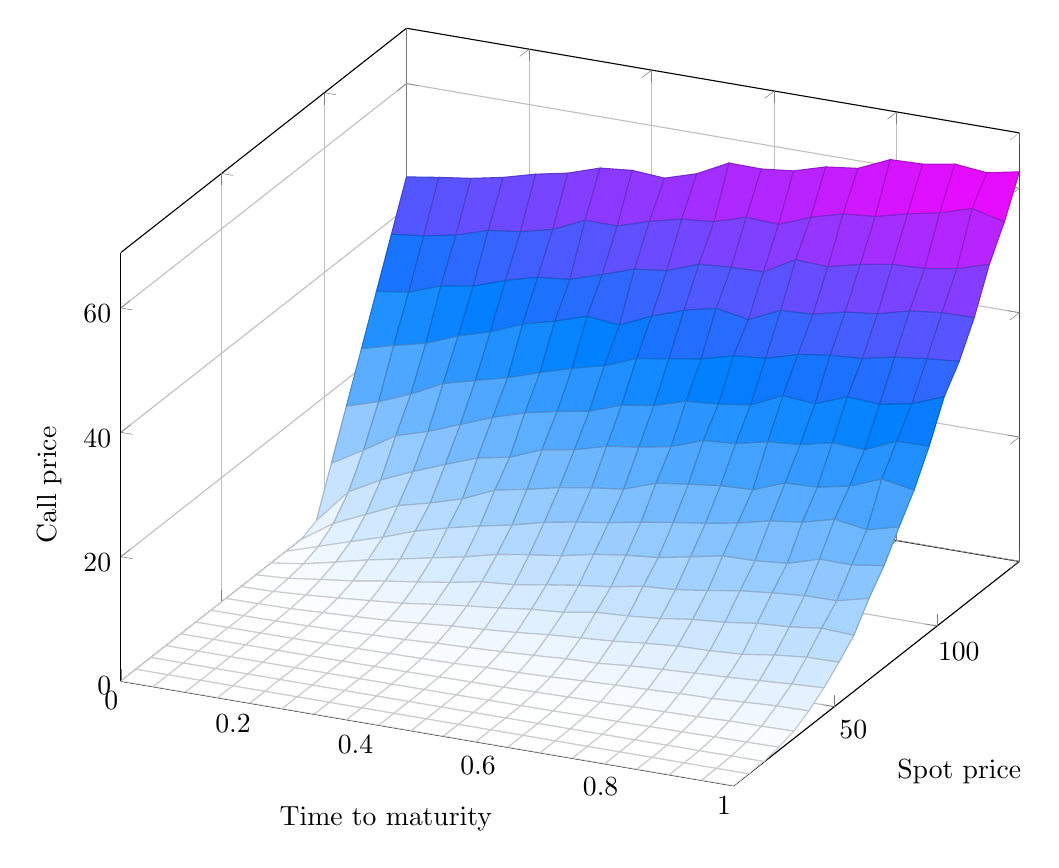
\begin{tikzpicture}
	\begin{axis}[
	% title={Call price surface $K=95$, $\lambda=4$, $\mu=0.05$, $\sigma=0.5$, $U\sim \mathcal{N}(0.05, 0.09)$}, 
	xlabel={$\mbox{Time to maturity}$},
    ylabel={$\mbox{Spot price}$},
    zlabel={$\mbox{Call price}$},
	colormap/cool,
	zmin=0,
	grid]
	\addplot3[surf,]
	 coordinates {
	(0.0, 1.0, 0.0) (0.05263157894736842, 1.0, 1.2711310619787809e-73) (0.10526315789473684, 1.0, 1.635945408240489e-40) (0.15789473684210525, 1.0, 2.311237689295037e-30) (0.21052631578947367, 1.0, 4.94118357581085e-29) (0.2631578947368421, 1.0, 1.482950176064908e-23) (0.3157894736842105, 1.0, 1.9519903745523e-18) (0.3684210526315789, 1.0, 2.266520652218845e-19) (0.42105263157894735, 1.0, 1.7552888447578743e-17) (0.4736842105263158, 1.0, 2.0364364601135484e-14) (0.5263157894736842, 1.0, 8.342706965191228e-12) (0.5789473684210527, 1.0, 5.4141165401698094e-12) (0.631578947368421, 1.0, 1.599701964159278e-09) (0.6842105263157894, 1.0, 6.532797872932028e-12) (0.7368421052631579, 1.0, 1.840639298701009e-11) (0.7894736842105263, 1.0, 2.642760831944296e-10) (0.8421052631578947, 1.0, 4.110016486439185e-11) (0.8947368421052628, 1.0, 1.2241867409004536e-10) (0.9473684210526316, 1.0, 8.514360091229447e-08) (1.0, 1.0, 9.315244361915646e-09) 

	(0.0, 8.315789473684209, 0.0) (0.05263157894736842, 8.315789473684209, 9.4818638581836e-12) (0.10526315789473684, 8.315789473684209, 2.7571182241389955e-08) (0.15789473684210525, 8.315789473684209, 1.8386560473914825e-07) (0.21052631578947367, 8.315789473684209, 3.3429961263146644e-07) (0.2631578947368421, 8.315789473684209, 5.833782187631924e-06) (0.3157894736842105, 8.315789473684209, 7.2842824361818615e-06) (0.3684210526315789, 8.315789473684209, 1.8067128361675247e-05) (0.42105263157894735, 8.315789473684209, 0.00020251954543196385) (0.4736842105263158, 8.315789473684209, 7.303029411200261e-05) (0.5263157894736842, 8.315789473684209, 0.00032434534431804817) (0.5789473684210527, 8.315789473684209, 0.0004030744394703346) (0.631578947368421, 8.315789473684209, 0.0009946857278088383) (0.6842105263157894, 8.315789473684209, 0.0013887007633734526) (0.7368421052631579, 8.315789473684209, 0.002432826247579628) (0.7894736842105263, 8.315789473684209, 0.002508228786162918) (0.8421052631578947, 8.315789473684209, 0.003340960883073069) (0.8947368421052628, 8.315789473684209, 0.004981093124723274) (0.9473684210526316, 8.315789473684209, 0.006534316226126668) (1.0, 8.315789473684209, 0.005542440273478858) 

	(0.0, 15.63157894736842, 0.0) (0.05263157894736842, 15.63157894736842, 1.7510910620861587e-07) (0.10526315789473684, 15.63157894736842, 3.7492994213456137e-06) (0.15789473684210525, 15.63157894736842, 2.6846812757352475e-05) (0.21052631578947367, 15.63157894736842, 0.0008149720285659335) (0.2631578947368421, 15.63157894736842, 0.00044511228909627714) (0.3157894736842105, 15.63157894736842, 0.0010666167106719536) (0.3684210526315789, 15.63157894736842, 0.003558713754242765) (0.42105263157894735, 15.63157894736842, 0.004989663596852301) (0.4736842105263158, 15.63157894736842, 0.01015263427767375) (0.5263157894736842, 15.63157894736842, 0.008690432856595542) (0.5789473684210527, 15.63157894736842, 0.017226582508587208) (0.631578947368421, 15.63157894736842, 0.019479189357613) (0.6842105263157894, 15.63157894736842, 0.03454517405111522) (0.7368421052631579, 15.63157894736842, 0.038162151371674335) (0.7894736842105263, 15.63157894736842, 0.045077664472836336) (0.8421052631578947, 15.63157894736842, 0.05953380601094568) (0.8947368421052628, 15.63157894736842, 0.0691157982444093) (0.9473684210526316, 15.63157894736842, 0.09847185313238133) (1.0, 15.63157894736842, 0.1061957517027669) 

	(0.0, 22.947368421052627, 0.0) (0.05263157894736842, 22.947368421052627, 5.084221030084646e-06) (0.10526315789473684, 22.947368421052627, 0.0001866731208782408) (0.15789473684210525, 22.947368421052627, 0.001138168047638918) (0.21052631578947367, 22.947368421052627, 0.002448966660330594) (0.2631578947368421, 22.947368421052627, 0.008857277203597679) (0.3157894736842105, 22.947368421052627, 0.012009149868726612) (0.3684210526315789, 22.947368421052627, 0.02585893417113413) (0.42105263157894735, 22.947368421052627, 0.03169914034282155) (0.4736842105263158, 22.947368421052627, 0.05243022081464221) (0.5263157894736842, 22.947368421052627, 0.07956615220755638) (0.5789473684210527, 22.947368421052627, 0.09664031259733892) (0.631578947368421, 22.947368421052627, 0.13526631547385287) (0.6842105263157894, 22.947368421052627, 0.19999994469712906) (0.7368421052631579, 22.947368421052627, 0.2091492209603374) (0.7894736842105263, 22.947368421052627, 0.27539521976457626) (0.8421052631578947, 22.947368421052627, 0.3217115737663569) (0.8947368421052628, 22.947368421052627, 0.3845700597342877) (0.9473684210526316, 22.947368421052627, 0.4413201038985207) (1.0, 22.947368421052627, 0.504890550021702) 

	(0.0, 30.26315789473684, 0.0) (0.05263157894736842, 30.26315789473684, 0.00021636824009878798) (0.10526315789473684, 30.26315789473684, 0.0017882370231065577) (0.15789473684210525, 30.26315789473684, 0.00716775354450988) (0.21052631578947367, 30.26315789473684, 0.01975918607235236) (0.2631578947368421, 30.26315789473684, 0.04874450193736063) (0.3157894736842105, 30.26315789473684, 0.07080961302888149) (0.3684210526315789, 30.26315789473684, 0.10465180326375344) (0.42105263157894735, 30.26315789473684, 0.15105792831627313) (0.4736842105263158, 30.26315789473684, 0.2267687926081301) (0.5263157894736842, 30.26315789473684, 0.2825723192389609) (0.5789473684210527, 30.26315789473684, 0.3739933070469711) (0.631578947368421, 30.26315789473684, 0.4750278753554938) (0.6842105263157894, 30.26315789473684, 0.5438405894870204) (0.7368421052631579, 30.26315789473684, 0.6795227070940679) (0.7894736842105263, 30.26315789473684, 0.7498510247091813) (0.8421052631578947, 30.26315789473684, 0.8476686739278232) (0.8947368421052628, 30.26315789473684, 1.048321061040062) (0.9473684210526316, 30.26315789473684, 1.0993835677771415) (1.0, 30.26315789473684, 1.1965468197751148) 

	(0.0, 37.578947368421055, 0.0) (0.05263157894736842, 37.578947368421055, 0.0021917242763076408) (0.10526315789473684, 37.578947368421055, 0.013259616221940902) (0.15789473684210525, 37.578947368421055, 0.030974470937349414) (0.21052631578947367, 37.578947368421055, 0.07355745025103849) (0.2631578947368421, 37.578947368421055, 0.16348489377861292) (0.3157894736842105, 37.578947368421055, 0.2484669383893498) (0.3684210526315789, 37.578947368421055, 0.33362297852338396) (0.42105263157894735, 37.578947368421055, 0.4358994515548125) (0.4736842105263158, 37.578947368421055, 0.6507078441280381) (0.5263157894736842, 37.578947368421055, 0.728730618367787) (0.5789473684210527, 37.578947368421055, 0.9136515018551707) (0.631578947368421, 37.578947368421055, 1.171710638308976) (0.6842105263157894, 37.578947368421055, 1.38668878159678) (0.7368421052631579, 37.578947368421055, 1.5592431151440334) (0.7894736842105263, 37.578947368421055, 1.7915773820548444) (0.8421052631578947, 37.578947368421055, 1.8869351524364868) (0.8947368421052628, 37.578947368421055, 2.177366528346691) (0.9473684210526316, 37.578947368421055, 2.461897962651922) (1.0, 37.578947368421055, 2.5418172276527233) 

	(0.0, 44.89473684210525, 0.0) (0.05263157894736842, 44.89473684210525, 0.008735629594718604) (0.10526315789473684, 44.89473684210525, 0.04869627581296259) (0.15789473684210525, 44.89473684210525, 0.14347825384390864) (0.21052631578947367, 44.89473684210525, 0.26026781675108296) (0.2631578947368421, 44.89473684210525, 0.4563272006082185) (0.3157894736842105, 44.89473684210525, 0.5973045078091729) (0.3684210526315789, 44.89473684210525, 0.8823334960698046) (0.42105263157894735, 44.89473684210525, 1.0900302283331185) (0.4736842105263158, 44.89473684210525, 1.3178891517037497) (0.5263157894736842, 44.89473684210525, 1.6045274439567796) (0.5789473684210527, 44.89473684210525, 1.944196025460392) (0.631578947368421, 44.89473684210525, 2.107769535163056) (0.6842105263157894, 44.89473684210525, 2.571239706382175) (0.7368421052631579, 44.89473684210525, 2.8743122242566965) (0.7894736842105263, 44.89473684210525, 3.1781428815264934) (0.8421052631578947, 44.89473684210525, 3.415127743768542) (0.8947368421052628, 44.89473684210525, 3.735004904507127) (0.9473684210526316, 44.89473684210525, 4.077055981411848) (1.0, 44.89473684210525, 4.359838736278544) 

	(0.0, 52.21052631578947, 0.0) (0.05263157894736842, 52.21052631578947, 0.041872517821787435) (0.10526315789473684, 52.21052631578947, 0.13769982164725506) (0.15789473684210525, 52.21052631578947, 0.3766765817407578) (0.21052631578947367, 52.21052631578947, 0.6225330383120853) (0.2631578947368421, 52.21052631578947, 0.9114837685872892) (0.3157894736842105, 52.21052631578947, 1.3214521013383949) (0.3684210526315789, 52.21052631578947, 1.7530629538004296) (0.42105263157894735, 52.21052631578947, 2.1072693138841463) (0.4736842105263158, 52.21052631578947, 2.496715090085148) (0.5263157894736842, 52.21052631578947, 3.0238450717882372) (0.5789473684210527, 52.21052631578947, 3.3989609641831433) (0.631578947368421, 52.21052631578947, 3.757717700575502) (0.6842105263157894, 52.21052631578947, 4.309817733117628) (0.7368421052631579, 52.21052631578947, 4.733592175450721) (0.7894736842105263, 52.21052631578947, 4.882879626986468) (0.8421052631578947, 52.21052631578947, 5.176456445150974) (0.8947368421052628, 52.21052631578947, 5.954931860741862) (0.9473684210526316, 52.21052631578947, 6.4972135071524715) (1.0, 52.21052631578947, 6.560795586389501) 

	(0.0, 59.526315789473685, 0.0) (0.05263157894736842, 59.526315789473685, 0.11947855107728292) (0.10526315789473684, 59.526315789473685, 0.4379665772350094) (0.15789473684210525, 59.526315789473685, 0.8472177841483102) (0.21052631578947367, 59.526315789473685, 1.292869532150536) (0.2631578947368421, 59.526315789473685, 1.7500052983542502) (0.3157894736842105, 59.526315789473685, 2.472881794521724) (0.3684210526315789, 59.526315789473685, 3.0953292215060277) (0.42105263157894735, 59.526315789473685, 3.657181436931309) (0.4736842105263158, 59.526315789473685, 4.324451494269348) (0.5263157894736842, 59.526315789473685, 4.72260516640344) (0.5789473684210527, 59.526315789473685, 5.607612402068952) (0.631578947368421, 59.526315789473685, 5.912459310128981) (0.6842105263157894, 59.526315789473685, 6.393244424556428) (0.7368421052631579, 59.526315789473685, 7.128688915407275) (0.7894736842105263, 59.526315789473685, 7.545753128652356) (0.8421052631578947, 59.526315789473685, 8.267577094980147) (0.8947368421052628, 59.526315789473685, 8.586885269312617) (0.9473684210526316, 59.526315789473685, 9.246960649628189) (1.0, 59.526315789473685, 9.017871946794992) 

	(0.0, 66.84210526315789, 0.0) (0.05263157894736842, 66.84210526315789, 0.3227618498965415) (0.10526315789473684, 66.84210526315789, 1.0315051473212196) (0.15789473684210525, 66.84210526315789, 1.6698715065370875) (0.21052631578947367, 66.84210526315789, 2.5513605721389907) (0.2631578947368421, 66.84210526315789, 3.2819634796064925) (0.3157894736842105, 66.84210526315789, 4.1032219970406585) (0.3684210526315789, 66.84210526315789, 5.078216717000778) (0.42105263157894735, 66.84210526315789, 5.500464690621111) (0.4736842105263158, 66.84210526315789, 6.359036858294664) (0.5263157894736842, 66.84210526315789, 7.164962478888725) (0.5789473684210527, 66.84210526315789, 7.821229705522678) (0.631578947368421, 66.84210526315789, 8.784641144207772) (0.6842105263157894, 66.84210526315789, 9.124428044641569) (0.7368421052631579, 66.84210526315789, 9.869173355295203) (0.7894736842105263, 66.84210526315789, 10.724596376114288) (0.8421052631578947, 66.84210526315789, 11.269169593893993) (0.8947368421052628, 66.84210526315789, 11.713048174703026) (0.9473684210526316, 66.84210526315789, 11.773766577430955) (1.0, 66.84210526315789, 13.042473247126356) 

	(0.0, 74.15789473684211, 0.0) (0.05263157894736842, 74.15789473684211, 0.7694513679180184) (0.10526315789473684, 74.15789473684211, 1.9243863078549013) (0.15789473684210525, 74.15789473684211, 3.1614385688600826) (0.21052631578947367, 74.15789473684211, 4.193986920589328) (0.2631578947368421, 74.15789473684211, 5.267550596448482) (0.3157894736842105, 74.15789473684211, 6.3030637729724655) (0.3684210526315789, 74.15789473684211, 7.583376762172028) (0.42105263157894735, 74.15789473684211, 8.424272786289674) (0.4736842105263158, 74.15789473684211, 9.134512569896026) (0.5263157894736842, 74.15789473684211, 10.257031825161482) (0.5789473684210527, 74.15789473684211, 10.993798365349264) (0.631578947368421, 74.15789473684211, 11.505843031067922) (0.6842105263157894, 74.15789473684211, 12.498030918632125) (0.7368421052631579, 74.15789473684211, 13.549208140730858) (0.7894736842105263, 74.15789473684211, 13.655461125253927) (0.8421052631578947, 74.15789473684211, 14.101368833433288) (0.8947368421052628, 74.15789473684211, 15.674531498019538) (0.9473684210526316, 74.15789473684211, 15.643330024792487) (1.0, 74.15789473684211, 16.40131350361768) 

	(0.0, 81.47368421052632, 0.0) (0.05263157894736842, 81.47368421052632, 1.66532288475349) (0.10526315789473684, 81.47368421052632, 3.3301839907163604) (0.15789473684210525, 81.47368421052632, 4.9287296621651855) (0.21052631578947367, 81.47368421052632, 6.773193007708594) (0.2631578947368421, 81.47368421052632, 8.170590812808829) (0.3157894736842105, 81.47368421052632, 9.359544571626152) (0.3684210526315789, 81.47368421052632, 10.409271627990671) (0.42105263157894735, 81.47368421052632, 11.729649629757777) (0.4736842105263158, 81.47368421052632, 12.65644204323275) (0.5263157894736842, 81.47368421052632, 13.437256275937465) (0.5789473684210527, 81.47368421052632, 14.405609869189096) (0.631578947368421, 81.47368421052632, 15.259618197000618) (0.6842105263157894, 81.47368421052632, 15.996755478511703) (0.7368421052631579, 81.47368421052632, 16.921830288601345) (0.7894736842105263, 81.47368421052632, 18.16473608078124) (0.8421052631578947, 81.47368421052632, 18.8276041690103) (0.8947368421052628, 81.47368421052632, 20.20027217125613) (0.9473684210526316, 81.47368421052632, 19.388549061373325) (1.0, 81.47368421052632, 20.720394285698866) 

	(0.0, 88.7894736842105, 0.0) (0.05263157894736842, 88.7894736842105, 3.4646892217616534) (0.10526315789473684, 88.7894736842105, 5.7796683586181965) (0.15789473684210525, 88.7894736842105, 8.10152754399534) (0.21052631578947367, 88.7894736842105, 9.398680349145927) (0.2631578947368421, 88.7894736842105, 10.955427520503902) (0.3157894736842105, 88.7894736842105, 13.232863840384006) (0.3684210526315789, 88.7894736842105, 14.243506584347436) (0.42105263157894735, 88.7894736842105, 15.410938157280526) (0.4736842105263158, 88.7894736842105, 16.263222437789054) (0.5263157894736842, 88.7894736842105, 16.933385640708636) (0.5789473684210527, 88.7894736842105, 18.780756411242596) (0.631578947368421, 88.7894736842105, 19.50066533077964) (0.6842105263157894, 88.7894736842105, 20.146214629635) (0.7368421052631579, 88.7894736842105, 20.38742627497396) (0.7894736842105263, 88.7894736842105, 22.347156629979462) (0.8421052631578947, 88.7894736842105, 22.546201714553646) (0.8947368421052628, 88.7894736842105, 23.626833942795887) (0.9473684210526316, 88.7894736842105, 25.656462782184896) (1.0, 88.7894736842105, 24.75864370032456) 

	(0.0, 96.10526315789473, 1.1052631578947398) (0.05263157894736842, 96.10526315789473, 6.650046310245742) (0.10526315789473684, 96.10526315789473, 9.424513737591292) (0.15789473684210525, 96.10526315789473, 11.687908192146688) (0.21052631578947367, 96.10526315789473, 13.691534726127488) (0.2631578947368421, 96.10526315789473, 15.618475798226664) (0.3157894736842105, 96.10526315789473, 16.626037027058132) (0.3684210526315789, 96.10526315789473, 18.730136952306584) (0.42105263157894735, 96.10526315789473, 19.596238158515643) (0.4736842105263158, 96.10526315789473, 21.04382379676384) (0.5263157894736842, 96.10526315789473, 21.78982484546801) (0.5789473684210527, 96.10526315789473, 22.76170922190678) (0.631578947368421, 96.10526315789473, 24.633803820417327) (0.6842105263157894, 96.10526315789473, 24.98955317619874) (0.7368421052631579, 96.10526315789473, 26.204663181340557) (0.7894736842105263, 96.10526315789473, 26.61508748478684) (0.8421052631578947, 96.10526315789473, 27.794652172642827) (0.8947368421052628, 96.10526315789473, 27.586982725121022) (0.9473684210526316, 96.10526315789473, 29.83007588651063) (1.0, 96.10526315789473, 29.899047472971525) 

	(0.0, 103.42105263157896, 8.421052631578945) (0.05263157894736842, 103.42105263157896, 11.44570865427468) (0.10526315789473684, 103.42105263157896, 14.646898820698901) (0.15789473684210525, 103.42105263157896, 16.206990740644418) (0.21052631578947367, 103.42105263157896, 18.224592020531308) (0.2631578947368421, 103.42105263157896, 20.23935731093179) (0.3157894736842105, 103.42105263157896, 21.86128159078204) (0.3684210526315789, 103.42105263157896, 22.97346589019933) (0.42105263157894735, 103.42105263157896, 23.904898222169447) (0.4736842105263158, 103.42105263157896, 25.762082073376426) (0.5263157894736842, 103.42105263157896, 26.58202498752677) (0.5789473684210527, 103.42105263157896, 28.15381286270244) (0.631578947368421, 103.42105263157896, 28.555440431660863) (0.6842105263157894, 103.42105263157896, 29.327546687660565) (0.7368421052631579, 103.42105263157896, 31.704509162914885) (0.7894736842105263, 103.42105263157896, 31.28922411761829) (0.8421052631578947, 103.42105263157896, 33.305526258526804) (0.8947368421052628, 103.42105263157896, 32.96717368562192) (0.9473684210526316, 103.42105263157896, 33.95537105111077) (1.0, 103.42105263157896, 35.97102680530655) 

	(0.0, 110.73684210526315, 15.736842105263165) (0.05263157894736842, 110.73684210526315, 17.318980405437447) (0.10526315789473684, 110.73684210526315, 19.45336497103148) (0.15789473684210525, 110.73684210526315, 22.02235625991425) (0.21052631578947367, 110.73684210526315, 23.40110304044491) (0.2631578947368421, 110.73684210526315, 24.734320511117872) (0.3157894736842105, 110.73684210526315, 26.430086621116146) (0.3684210526315789, 110.73684210526315, 28.00146860781445) (0.42105263157894735, 110.73684210526315, 29.31808866926424) (0.4736842105263158, 110.73684210526315, 31.35796189544785) (0.5263157894736842, 110.73684210526315, 32.197307346927) (0.5789473684210527, 110.73684210526315, 33.060911000948) (0.631578947368421, 110.73684210526315, 34.45734339748655) (0.6842105263157894, 110.73684210526315, 34.932739646458025) (0.7368421052631579, 110.73684210526315, 36.424621272641055) (0.7894736842105263, 110.73684210526315, 37.20479364177014) (0.8421052631578947, 110.73684210526315, 37.54720675045479) (0.8947368421052628, 110.73684210526315, 38.679113998573776) (0.9473684210526316, 110.73684210526315, 39.28847446694176) (1.0, 110.73684210526315, 39.75173086041486) 

	(0.0, 118.05263157894736, 23.052631578947373) (0.05263157894736842, 118.05263157894736, 24.47725681963611) (0.10526315789473684, 118.05263157894736, 25.723788325539907) (0.15789473684210525, 118.05263157894736, 27.770269835112373) (0.21052631578947367, 118.05263157894736, 29.32815351372659) (0.2631578947368421, 118.05263157894736, 31.443721087977337) (0.3157894736842105, 118.05263157894736, 32.805786327416115) (0.3684210526315789, 118.05263157894736, 34.478641020090265) (0.42105263157894735, 118.05263157894736, 33.93214597197779) (0.4736842105263158, 118.05263157894736, 36.27638363448385) (0.5263157894736842, 118.05263157894736, 38.085540913935645) (0.5789473684210527, 118.05263157894736, 39.30815637039815) (0.631578947368421, 118.05263157894736, 38.36466337538987) (0.6842105263157894, 118.05263157894736, 40.73749182381604) (0.7368421052631579, 118.05263157894736, 40.98895011270465) (0.7894736842105263, 118.05263157894736, 42.24437005388789) (0.8421052631578947, 118.05263157894736, 42.8324693090093) (0.8947368421052628, 118.05263157894736, 44.193682033269376) (0.9473684210526316, 118.05263157894736, 44.79216707498119) (1.0, 118.05263157894736, 44.908172103139755) 

	(0.0, 125.36842105263158, 30.368421052631568) (0.05263157894736842, 125.36842105263158, 31.14307388299269) (0.10526315789473684, 125.36842105263158, 33.044866045639004) (0.15789473684210525, 125.36842105263158, 33.88206628908602) (0.21052631578947367, 125.36842105263158, 35.68023355494522) (0.2631578947368421, 125.36842105263158, 37.08099156598556) (0.3157894736842105, 125.36842105263158, 37.63197252695679) (0.3684210526315789, 125.36842105263158, 39.29065892104133) (0.42105263157894735, 125.36842105263158, 41.044837685077894) (0.4736842105263158, 125.36842105263158, 41.680868224878424) (0.5263157894736842, 125.36842105263158, 43.61822200073408) (0.5789473684210527, 125.36842105263158, 43.996291123576185) (0.631578947368421, 125.36842105263158, 44.139368767053405) (0.6842105263157894, 125.36842105263158, 46.978708737927924) (0.7368421052631579, 125.36842105263158, 46.74549330381504) (0.7894736842105263, 125.36842105263158, 48.00198637536718) (0.8421052631578947, 125.36842105263158, 48.89879028542059) (0.8947368421052628, 125.36842105263158, 49.112615365636934) (0.9473684210526316, 125.36842105263158, 49.99809928854054) (1.0, 125.36842105263158, 51.53104208953643) 

	(0.0, 132.68421052631578, 37.68421052631578) (0.05263157894736842, 132.68421052631578, 38.29880924852953) (0.10526315789473684, 132.68421052631578, 39.308035192437785) (0.15789473684210525, 132.68421052631578, 40.95427651016865) (0.21052631578947367, 132.68421052631578, 41.627571022201415) (0.2631578947368421, 132.68421052631578, 42.87219676466616) (0.3157894736842105, 132.68421052631578, 45.22166570868122) (0.3684210526315789, 132.68421052631578, 45.20634630183278) (0.42105263157894735, 132.68421052631578, 46.82499410732114) (0.4736842105263158, 132.68421052631578, 48.082351088545934) (0.5263157894736842, 132.68421052631578, 48.54680945140389) (0.5789473684210527, 132.68421052631578, 50.15018296794618) (0.631578947368421, 132.68421052631578, 49.879717346952575) (0.6842105263157894, 132.68421052631578, 51.90208194077403) (0.7368421052631579, 132.68421052631578, 53.3439954769466) (0.7894736842105263, 132.68421052631578, 53.790253567599315) (0.8421052631578947, 132.68421052631578, 55.10357739597097) (0.8947368421052628, 132.68421052631578, 56.18514362801418) (0.9473684210526316, 132.68421052631578, 57.731094591065435) (1.0, 132.68421052631578, 56.48038834932546) 

	(0.0, 140.0, 45.0) (0.05263157894736842, 140.0, 45.81252287232222) (0.10526315789473684, 140.0, 46.536216715358236) (0.15789473684210525, 140.0, 47.57426461759381) (0.21052631578947367, 140.0, 48.97949056065039) (0.2631578947368421, 140.0, 50.02805541722807) (0.3157894736842105, 140.0, 51.72842002377443) (0.3684210526315789, 140.0, 52.24965596903553) (0.42105263157894735, 140.0, 51.88624310906413) (0.4736842105263158, 140.0, 53.47628997400301) (0.5263157894736842, 140.0, 56.0835801333374) (0.5789473684210527, 140.0, 56.01248546959969) (0.631578947368421, 140.0, 56.5897055996124) (0.6842105263157894, 140.0, 58.11162383508184) (0.7368421052631579, 140.0, 58.76613982638835) (0.7894736842105263, 140.0, 61.06105949771953) (0.8421052631578947, 140.0, 61.22397969695306) (0.8947368421052628, 140.0, 62.106054032026215) (0.9473684210526316, 140.0, 61.60121530819344) (1.0, 140.0, 62.64101580240984) 

	};
	\end{axis}
	\end{tikzpicture}
\caption{Call price surface $K=95$, $\lambda=4$, $\mu=0.05$, $\sigma=0.5$, $U\sim \mathcal{N}(0.05, 0.09)$}
\label{fig:call_surface}
\end{figure}


\chapter{Hedging}
% what is a local martingale?
% galtchouk kunita watanabe decomposition

Hedging is an investment made with the incentive of reducing the risk of adverse price movements in an asset. Usually, this is done by taking an offsetting (opposite) position in a related security. Indeed, we have already done that when we were constructing a hedging portfolio to price our option. Investors may consider hedging in order to manage their exposure to risk. Hedging is, of course, no free-lunch and it comes with a cost. While the benefit of hedging is that it allows us to reduce the risk, it also reduces the potential gains made by the investment. If an investor is facing uncertain market conditions and his positions are not hedged, the potential gains are high, but so are the potential losses. By hedging his positions to mitigate the risk, an investor has to accept the face the fact that the potential gains will scale down as well. 
In section \ref{sec:delta_hedge} we have already illustrated how to determine the quantity of the stock that we have to hold to hedge a position in an option written on that stock. The method we used there is called a \textit{delta hedge} ($\Delta$-hedge). 

\section{Delta hedging in Black-Scholes world}
Before diving into the process of hedging our option written on the stock which is governed by the jump-diffusion process, let us first take a step into the Black-Scholes world where we have \textit{ideal market conditions}:

\begin{enumerate}[label=(\roman*)]
	\item the risk free interest rate is known and is constant through time
	\item the stock price is governed by the geometric Brownian motion $$dX_t = \mu_t X_t dt + \sigma_t X_t dW_t$$
	\item the stock pays no dividend
	\item the market is \textit{frictionless}, that is, there are no transaction costs
	\item it is possible to borrow or deposit any amount of money at the risk free interest rate
	\item there are no penalties for shot selling
\end{enumerate}
Our starting point was the assumption that the option price will depend on the underlying asset price, that is: $$f_t = f(X_t)$$ Later we have arrived derived that in order to hedge a short position of $1$ option we would have to hold the amount $s$ of the underlying asset, where $s$ is 
\begin{equation} \label{eqn:s_delta}
	s = \frac{d}{dX_t}f(X_t)
\end{equation}
This means that if we would hold any time $t$ this amount of the underlying, our position would be perfectly hedged. In practice, however, continuous hedging is not possible. The best we can do is to choose specific points in time at which we would rebalance our portfolio. The more rebalancing times we have, the closer we get to the continuous hedging. The effect of hedging on the value of the portfolio will be investigated soon. Let us now examine on Figure \ref{fig:gbm_price_process} a generated asset price process, together with the price process of its call option that matures at time $T=1$ and has a strike price $K=120$. As we are still in the Black-Scholes world there is an absence of jumps and the underlying process is a pure geometric Brownian motion.

\begin{figure}[ht]
\centering
	\begin{tikzpicture}
	\begin{axis}[
	    % title={Price of the European Call Option that matures at $T=1$ with $K=100$, $r=2\%$},
	    xlabel={t},
	    ylabel={Price},
	    xmin=0, xmax=1,
	    % ymin=90, ymax=210,
	    ymajorgrids=true,
	    grid style=dashed,
	    legend pos=north east,
	]
	\addplot[color=olive] table[x index=0, y index=1] {data/gbm_hedging_results.dat};
	\addplot[color=magenta] table[x index=0, y index=2] {data/gbm_hedging_results.dat};
	\addplot[very thick, dashed, domain=0:1.0,gray] {120};
	% \addplot[color=magenta] table {data/jump_diffusion_process_falling.dat};
	\addlegendentry{Asset price}
	\addlegendentry{Call option price}
	\addlegendentry{Strike price}

	\end{axis}
	\end{tikzpicture}

\caption{Asset price governed by the geometric Brownian motion and call option price with $K=120$}
\label{fig:gbm_price_process}	
\end{figure}
\noindent Suppose we wrote (shorted) one call option at time $t=0$ and we want to hedge our position as we are unsure of the future price movements. In order for our position to be perfectly hedged we want to have $s$ units of the underlying asset, but to calculate $s$ we have to be able to differentiate the option price $f$ with respect to the process $X$. Luckily, this was already done in the original \cite{black_pricing_nodate} paper. Namely, the expression for obtaining the price of a call option is:

\begin{equation} \label{eqn:bs_call}
	C_t = X_tN(d_1) - N(d_2)Ke^{-r\tau}
\end{equation}
where
\begin{align*}
	C_t &- \mbox{call price at time } t \\
	X_t &- \mbox{price of the underlying asset at time } t \\
	\tau &- \mbox{time to maturity} \\
	K &- \mbox{strike price} \\
	r &- \mbox{risk-free rate} \\
	N &- \mbox{cumulative distribution function of } \mathcal{N}(0,1) \\
\end{align*}
and the terms $d_1$ and $d_2$ are

\begin{equation} \label{eqn:d1d2}
	d_1 = \frac{\ln{\frac{X_t}{K}} + \left(r + \frac{\sigma^2}{2} \right)\tau}{\sigma\sqrt{\tau}} \hspace{2cm} d_2 = d_1 - \sigma\sqrt{\tau}
\end{equation}
As the underlying asset price follows geometric Brownian motion we can use the expression \ref{eqn:bs_call} to obtain the call option price at each time $t$. The result can be observed in the Figure \ref{fig:gbm_price_process}. If we were to differentiate the above expression for $C$ with respect to $X$ we would obtain (for details refer to \ref{sec:obtain_delta_hedge}): 
\begin{equation} \label{eqn:delta_nd1}
	\frac{\partial C}{\partial X} = N(d_1)
\end{equation}
Combining this expression with the expression \ref{eqn:s_delta} we obtain that the number of assets we have to hold at each time $t$ is $N(d_1)$. Now we have all ingredients to be able to simulate and show hedging results. To illustrate the results, we set the initial portfolio value to be $50$ and we already know that we are short one call option, that means that our position in that option is $-1$. We are considering the process shown at Figure \ref{fig:gbm_price_process} and we will perform delta hedging with different number of rebalancing times. On Figure \ref{fig:hedging_gbm} one can observe the effect of hedging with different number of rebalancing times. The first rebalancing time occurs at time $t=0$. 

\begin{figure}[ht]
\centering
	\begin{tikzpicture}
	\begin{axis}[
	    % title={Price of the European Call Option that matures at $T=1$ with $K=100$, $r=2\%$},
	    xlabel={t},
	    ylabel={Portfolio value},
	    xmin=0, xmax=1,
	    % ymin=90, ymax=210,
	    ymajorgrids=true,
	    grid style=dashed,
	    legend pos=south west,
	]
	\addplot[semithick, color=olive] table[x index=0, y index=3] {data/gbm_hedging_results.dat};
	\addplot[semithick, color=magenta] table[x index=0, y index=4] {data/gbm_hedging_results.dat};
	\addplot[semithick, color=teal] table[x index=0, y index=5] {data/gbm_hedging_results.dat};
	\addplot[semithick, color=orange] table[x index=0, y index=6] {data/gbm_hedging_results.dat};
	% \addplot[color=magenta] table {data/jump_diffusion_process_falling.dat};
	\addlegendentry{$n = 1$}
	\addlegendentry{$n = 2$}
	\addlegendentry{$n = 5$}
	\addlegendentry{$n = 10$}

	\end{axis}
	\end{tikzpicture}

\caption{Development of the portfolio value with initial value of $50$ for different number of rebalancing times $n$}
\label{fig:hedging_gbm}	
\end{figure}
By frequently rebalancing our portfolio we ensure the stability in the value of our portfolio. This can be further examined if we were to plot the distributions of portfolio value at time $t=T$ for different numbers of rebalancing times. This is shown on the Figure (\ref{fig:portfolio_value_distribution}).

\begin{figure}[ht]
\centering
	\begin{tikzpicture}
	\begin{axis}[
	    % title={Price of the European Call Option that matures at $T=1$ with $K=100$, $r=2\%$},
	    xlabel={Portfolio value at $t=T$},
	    % ylabel={Price},
	    xmin=38, xmax=65,
	    ymajorgrids=true,
	    grid style=dashed,
	    legend pos=north west,
	]
	% \addplot[thick, color=olive] table[x index=0, y index=1] {data/gbm_hedging_distributions.dat};
	% \addplot[thick, color=magenta] table[x index=2, y index=3] {data/gbm_hedging_distributions.dat};
	\addplot[thick, dashed, color=gray] table[x index=4, y index=5] {data/gbm_hedging_distributions.dat};
	\addplot[thick, dashed, color=orange] table[x index=6, y index=7] {data/gbm_hedging_distributions.dat};
	\addplot[thick, dashed, color=blue] table[x index=8, y index=9] {data/gbm_hedging_distributions.dat};
	\addplot[thick, dashed, color=purple] table[x index=10, y index=11] {data/gbm_hedging_distributions.dat};
	\addplot[thick, dashed, color=teal] table[x index=12, y index=13] {data/gbm_hedging_distributions.dat};
	% \addplot[color=magenta] table {data/jump_diffusion_process_falling.dat};
	% \addlegendentry{$n = 1$}
	% \addlegendentry{$n = 2$}
	\addlegendentry{$n = 4$}
	\addlegendentry{$n = 10$}
	\addlegendentry{$n = 50$}
	\addlegendentry{$n = 100$}
	\addlegendentry{$n = 500$}

	\end{axis}
	\end{tikzpicture}

\caption{Portfolio value distributions at time $t=T$ for different numbers of rebalancing times $n$}
\label{fig:portfolio_value_distribution}	
\end{figure}

\section{Quadratic hedging of contingent claims}
When we were showing that a regular Black-Scholes delta hedge in case of a jump-diffusion model cannot eliminate jump risk we stopped there. In fact in \cite{chiarella_derivative_2015} the autors demonstrate that in case we have a finite number $n$ of jump amplitudes, we can hedge away the jump risk by using $n$ additional derivative securities with different strike prices and maturities. In our case the jump amplitude is normally distributed, that is, there is an infinite number of different jump sizes and we would need an infinite number of different derivative securities to hedge away the jump risk. This is not possible and that means that a contingent claim cannot be perfectly replicated and according to the Theorem \ref{tm:ftap2} we have an \textbf{incomplete market} situation. Since there will always exist some amount of hedging error the best we can do is to try and minimize that error, this leads us to investigate other hedging techniques, one of which is quadratic hedging. Moreover, in this section we will also have a look at how to mathematically define a problem of hedging. For that we will need to introduce a notion of a \textit{trading strategy}. Although we have not defined it explicitly, we have already used it. A \textbf{trading strategy} is simply our selection of a covering portfolio in the underlying asset. \cite{bingham_risk-neutral_2004} define it as

\begin{definition}
	Denote by L(X) the linear space of all $\mathbb{R}^d$-valued predictable $X$-integrable processes $\phi$. A self-financing trading strategy is any pair $(V_0, \phi)$ such that $V_0$ is and $\mathcal{F}_0$-measurable random variable and $\phi \in L(X)$.
\end{definition}
\noindent A value $\phi^i(t)$ can be interpreted of as a number of shares of asset $i$ held at time $t$ and $V_0$ is the initial capital of an investor. By choosing a covering portfolio, we generate a value process, which is used to cover our exposure. Its value is given by

\begin{equation}
	V_t(\phi) := V_0 + \int_0^t \phi(u) dX_u
\end{equation} 
And the gains made from the trading process up to time $t$ is denoted by $G_t(\phi)=\int_0^t \phi(u)dX_u$. When we choose a trading strategy and the initial capital we can then think about how to evaluate the trading strategy. At time $T$ the contingent claim will have a payoff of $H$ and our carefully chosen portfolio will have a value of $V_T(\phi)$. To asses the quality of the trading strategy we will use the difference of those 2 quantities. To be more specific, we will calculate the hedging error as the square of that difference - quadratic loss function. \cite{bingham_risk-neutral_2004} give in their book the definition of mean-variance strategy to hedge $H$ (Definition \ref{def:mean_variance_hedge}). So far, we have mentioned a term \textit{risk} multiple times and it is mostly clear what it means, but it may be unclear how to measure it. There are various ways of quantifying risk. One such is to quantify it represent it through the variance of returns. Logically, if we have a process with low variance, this means that the probability of a process steering far away from its expected value is low. Analogously, for a high-variance process we can with less certainty predict its movements and future paths. This is the core idea of hedging methods that aim to reduce the risk of the future payoff.

\begin{definition} \label{def:mean_variance_hedge}
	Let $\Phi$ be a the space of all $\phi \in L(X)$ for which $G_T(\phi)$ is in $L^2(\mathbb{P})$ and the gains from the trading process $G_t(\phi)$ is a martingale under the probability measure $\tilde{\mathbb{P}}$. A pair $(V_0, \phi)$ such that $V_0 \in \mathbb{R}$ and $\phi \in \Phi$ is called a mean-variance optimal strategy for $H$, if it solves the optimization problem 
	\begin{equation} \label{eqn:min_hedge_error}
		\min_{\phi}\mathbb{E}\left[ (H - V_0 - G_T(\phi))^2 \right]
	\end{equation}
\end{definition}
In case when there is an absence of jumps, that is, we are in the Black-Scholes world, the solution to this optimization problem is simply sensitivity of the option price with respect to the underlying asset price
\begin{equation*}
	\frac{\partial C}{\partial X} = N(d_1)
\end{equation*}
In case there is an absence of diffusion and we are left with only jump process with only 1 possible jump amplitude, the solution is:
\begin{equation} \label{eqn:delta_no_diffusion}
	\phi^* = \frac{C(X_t + k) - C(X_t)}{k}
\end{equation}
To illustrate why, we look at the time $t$ and observe an asset price $X_t$ and a price of the call option $C(X_t)$ on that asset. We know that at time $t+dt$ a process can either stay the same or jump, where the size of the jump has a single possible value $k$. We denote the value of our portfolio at time $t$ with $$V_t = \phi^* X_t - C(X_t)$$ if the jump arrives inside the time interval $dt$ the value of out portfolio will be
$$V_{t+dt} = \phi^* (X_t + k) - C(X_t + k)$$
and if the jump does not arrive the asset price will stay the same and the price of the call option will change by only marginal amount (because we are closer to the maturity), which can be ignored. This means that the value of our portfolio, in this case, has virtually stayed unchanged no matter the value of $\phi^*$. If we want the value of our portfolio to stay unchanged also in presence of jump inside the time interval $dt$ we have to choose $\phi^*$ wisely.
\begin{align*}
	V_t &= V_{t+dt} \\
	X_t\phi^* - C(X_t) &=  X_t\phi^*+ k\phi^* - C(X_t + k) \\
	k\phi^* &= C(X_t + k) - C(X_t)
\end{align*} and we arrive to the final formula (\ref{eqn:delta_no_diffusion}).

\noindent The derivation of the solution to the optimization problem \ref{eqn:min_hedge_error} goes beyond the scope of this thesis and is rather cumbersome. In turn, we will present the solution for the problem obtained in \cite{cont_financial_2004}:
\begin{equation} \label{eqn:quadratic_hedge}
	\phi^* = \frac{\sigma^2 \frac{\partial C}{\partial X} + \frac{1}{X} \int z[C(t,X(1+z))-C(t,X)] \nu_U(z)dz}{\sigma^2 + \int z^2 \nu_U(z)dz}
\end{equation} where $C(t,X)$ is the Black-Scholes price for the call option and accordingly the $\frac{\partial C}{\partial X}$ is the sensitivity of that price with respect to the price of the underlying asset. The function $\nu_U$ is the probability density function of the jump size $U$. This result can be interpreted as the average of the simple $\Delta$-hedge in the absence of jumps and the $\Delta$-hedge in case there is no diffusion part (\ref{eqn:delta_no_diffusion}). To check the effectiveness of the quadratic hedge, we will first use the jump-diffusion process on figure \ref{fig:call_price1} and compare the performance of the quadratic hedge and the regular $\Delta$-hedge, where we pretend that the underlying process has only diffusion component without jumps. 

\begin{figure}[ht]
\centering
	\begin{tikzpicture}
	\begin{axis}[
	    % title={Price of the European Call Option that matures at $T=1$ with $K=100$, $r=2\%$},
	    xlabel={t},
	    ylabel={Portfolio value},
	    xmin=0, xmax=1,
	    ymin=30, ymax=70,
	    ymajorgrids=true,
	    grid style=dashed,
	    legend pos=north west,
	]
	\addplot[semithick, color=magenta] table[x index=0, y index=1] {data/one_process_hedging_comparison.csv};
	\addplot[semithick, color=teal] table[x index=0, y index=2] {data/one_process_hedging_comparison.csv};
	\addplot[dotted] coordinates {(0.019759280317646837,0) (0.019759280317646837,218.87657564987035)};
	\draw[dotted] (axis cs:0.4804255332905141,0) -- (axis cs:0.4804255332905141,218.87657564987035);
	\draw[dotted] (axis cs:0.4878563562516914,0) -- (axis cs:0.4878563562516914,218.87657564987035);
	\draw[dotted] (axis cs:0.5769236248364072,0) -- (axis cs:0.5769236248364072,218.87657564987035);
	\draw[dotted] (axis cs:0.6785902080596808,0) -- (axis cs:0.6785902080596808,218.87657564987035);
	\addlegendentry{$\Delta$-hedge}
	\addlegendentry{Quadratic hedge}
	\addlegendentry{Jump times}
	\end{axis}
	\end{tikzpicture}

\caption{Development of the portfolio value with initial value of $50$ for two different hedging strategies}
\label{fig:hedging_jump_diffusion}	
\end{figure}

\noindent On Figure \ref{fig:hedging_jump_diffusion}, in terms of stability, both processes seem to be similar and we even observe a lower final value of the portfolio with quadratic hedging. Let us remember that profit is not the goal of hedging, but rather a method to preserve the value of the portfolio over time. With this in mind, one possible way to measure success of a hedging method is the absolute difference from the initial portfolio value remunerated at the risk free rate $r$. This means, if the portfolio value is initially set to $V$, the expected value at maturity is $V\cdot e^{rT}$. Continuing further, we will now compare the performance of both hedging methods on 30 different jump-diffusion processes. Generated processes had the following characteristics: 

\begin{table}
\centering
\begin{tabular}{c c c}
\hline
Symbol & Description & Value \\
\hline \hline
$X_0$ & initial asset price & $100$ \\
\hline
$\mu$ & asset price drift & $0.05$ \\
\hline
$\sigma$ & asset price volatility & $0.5$ \\
\hline
$\lambda$ & jump intensity & $4$ \\
\hline
$r$ & risk free rate & $0.02$ \\
\hline
$K$ & call option strike price & $100$ \\
\hline
$U$ & jump size distribution & $\mathcal{N}(\mu=0.05, \sigma^2 = 0.22^2)$ \\
\hline
$T$ & option maturity & $1$ \\
\hline
\end{tabular}
\caption{Jump-diffusion process characteristics}
\end{table}


A table with final values of the portfolio can be seen in Appendix \ref{appendix:section_tables}. To obtain a numerical comparison between the two hedging methods we perform a paired t-test, as the two methods are not independent. They are related through the generated processes. We quantify the success of each portfolio as the absolute distance from final value of the  risk-free portfolio with the same initial value. We want to test whether the value absolute difference of the quadratically hedged portfolio is lower than the absolute difference of the $\Delta$-hedged portfolio. By setting up this one-sided alternative, we obtain a p-value of $0.7366$. In other words, there is no evidence that the quadratic hedge does a better job than a classic $\Delta$-hedge. It is, in fact, even more leaned towards the side of the $\Delta$-hedge doing a better job. One could argue that by increasing the jump intensity our quadratic hedge could really shine. The reason for that is that the path of a process with lower intensity has a higher probability of being \textit{closer} to the path generated by a regular geometric Brownian motion. Further improvements could be made to tune the jump intensity parameter and jump size distribution to mimic the real world as closely as possible, and perform this analysis again. Nevertheless, by introducing the quadratic hedging we have obtained a new, very capable, tool which could in future help us hedge our portfolios in presence of processes with jump characteristics.

\chapter{Conclusion}
We have undergone a journey starting from the basic financial concepts and establishing a process that will model a price of an asset, through pricing an option that derives its value from this asset and finally we have shown how to hedge such a contingent claim. The theory of derivatives market is more concerned about the relationship between the underlying and its derivative and much less with economic fundamentals that determine the price of the underlying. However, some basic economic reasoning and concepts have to be incorporated, but the focus is on the mathematical formulation. 

We have constructed a mathematical model of real markets, which is of course still a simplification. Nevertheless, it allowed us to draw some useful conclusions, for example, why the premium requested by the writer of the option is equal to the expected value of the discounted future payoff of the option. Furthermore, we have seen that by increasing the average number of jumps (parameter $\lambda$) the price of the option increased as a consequence of the fact that an option has a higher probability of ending up in-the-money. Like we have already mentioned, the Black-Scholes model of stock prices does not take into account the potential jumps that, in real world, occur due to some political or economical events and are not predictable. What this entails is if we were to use Black-Scholes model to price options, we may end up with underpriced options and there may exist an arbitrage opportunity. The similar goes for hedging.

Further improvements of this work are naturally possible. For example, one could incorporate stochastic processes that will model volatility and risk-free rate, both of which have been kept constant in the our work so far. Nonetheless, we have created a decent model of the market with less constraints than the one proposed by \cite{black_pricing_1972}. By doing this, we have taken a serious step into derivative pricing, a field that has a lot of ideas still left to explore. Hopefully, this thesis has given a reader a thourough overview of the main ideas in mathematical finance and derivative pricing which forms a stable foundation for further exploration in the field. 

\bibliography{bibliography}
% Use zotero for this
\bibliographystyle{fer}
\nocite{*}

\listoffigures

\newpage
\begin{abstract}
Stochastic processes have a widespread application in the computer science and in this thesis their application in the field of finance will be studied. The focus of this thesis will be to mathematically define a price of an asset using a jump-diffusion model which is then used to price a derivative. By programming simulations of prices of an asset and its derivative, their behaviour in time will be shown. After the prices of an asset and its derivative have been defined, we want to show how to mathematically define a problem of hedging a position. This also has to be accompanied with implemented simulations to illustrate the effect of hedging.

\keywords{stochastic processes, finance, pricing, options, hedging}
\end{abstract}

\hrvtitle{Određivanje cijene i premošćivanja rizika u slučaju difuzijskog procesa sa skokovima}
\begin{sazetak}
Stohastički procesi imaju široku primjenu u raznim područjima računarske znanosti, a u sklopu ovog rada istražit će se njihova primjena u području financija. Fokus rada je matematički definirati proces cijene nekog sredstva u obliku difuzijskog procesa sa skokovima, na temelju kojeg se naknadno određuje cijena njegovog financijskog derivata. Potrebno je programskim simulacijama cijena sredstva i derivata pokazati njihovo ponašanje u vremenu. Nakon što su spomenuti procesi cijena definirani, želimo pokazati kako se matematički može predstaviti i riješiti problem premošćivanja rizika, te navedeno popratiti programskim simulacijama scenarija s ciljem ilustracije efekta premošćivanja rizika.

\kljucnerijeci{stohastički procesi, financije, određivanje cijene, opcije, premošćivanje rizika}
\end{sazetak}

\appendix
\chapter{Tables and derivations}
\section{Delta hedge} \label{sec:obtain_delta_hedge}

Starting from \ref{eqn:bs_call} and \ref{eqn:d1d2} we want to obtain the expression \ref{eqn:delta_nd1}. Of course we just need to differentiate the call price by $X$, but also $d_1$ and $d_2$ are functions of $X$ and it is maybe not immediately straighforward how to obtain the expression \ref{eqn:delta_nd1}. 
\begin{equation*}
	C_t = X_tN(d_1) - N(d_2)Ke^{-r\tau} \hspace{0.5cm} \Big/ \frac{\partial}{\partial X}
\end{equation*}
\begin{equation*}
	\frac{\partial C}{\partial X} = \frac{\partial}{\partial X}\left[ XN(d_1) \right] - \frac{\partial}{\partial X} \left[ N(d_2)Ke^{-r\tau} \right]
\end{equation*}
\begin{equation} \label{eqn:dC_dX}
	\frac{\partial C}{\partial X} = N(d_1) + X\frac{\partial N(d_1)}{\partial X} - Ke^{-r\tau}\frac{\partial N(d_2)}{\partial X}
\end{equation} Now we will decompose the terms $\frac{\partial N(d_1)}{\partial X}$ and $\frac{\partial N(d_2)}{\partial X}$, but first let us take a look at what $N(z)$ represents. $N$ is a unit normal cumulative distribution function, that is:
\begin{equation} 
	N(z) = \frac{1}{\sqrt{2\pi}} \int_{-\infty}^{z} e^{-\frac{u^2}{2}}du
\end{equation} which means that the $\frac{\partial N}{\partial z}$ is the value of the unit normal probability density function at the point $z$ or in our case this would mean:
\begin{equation}
	\frac{\partial N}{\partial d_1} = \frac{1}{\sqrt{2\pi}} e^{-\frac{d_1^2}{2}} \hspace{0.5cm} \mbox{and} \hspace{0.5cm} \frac{\partial N}{\partial d_2} = \frac{1}{\sqrt{2\pi}} e^{-\frac{d_2^2}{2}}
\end{equation} We also repeat expressions for $d_1$ and $d_2$:

\begin{equation*}
	d_1 = \frac{\ln{\frac{X_t}{K}} + \left(r + \frac{\sigma^2}{2} \right)\tau}{\sigma\sqrt{\tau}} \hspace{2cm} d_2 = d_1 - \sigma\sqrt{\tau}
\end{equation*} Let us now go back to $\frac{\partial N(d_1)}{\partial X}$ and $\frac{\partial N(d_2)}{\partial X}$ we obtain the following expression for $\frac{\partial N(d_1)}{\partial X}$:
\begin{equation*}
	\frac{\partial N(d_1)}{\partial X} = \frac{\partial N}{\partial d_1} \frac{\partial d_1}{\partial X} = \frac{1}{\sqrt{2\pi}}e^{-\frac{d_1^2}{2}}\frac{1}{\sigma\sqrt{\tau}}\frac{K}{X}\frac{1}{K}
\end{equation*}
\begin{equation}
	\frac{\partial N(d_1)}{\partial X} = \frac{1}{X\sigma\sqrt{2\pi\tau}}e^{-\frac{d_1^2}{2}}
\end{equation} and analoguously for $d_2$
\begin{equation*}
	\frac{\partial N(d_2)}{\partial X} = \frac{1}{X\sigma\sqrt{2\pi\tau}}e^{-\frac{d_2^2}{2}} = \frac{1}{X\sigma\sqrt{2\pi\tau}}e^{-\frac{(d_1 - \sigma\sqrt{\tau})^2}{2}}
\end{equation*}
\begin{equation}
	\frac{\partial N(d_2)}{\partial X} = \frac{1}{X\sigma\sqrt{2\pi\tau}}e^{-\frac{d_1^2}{2}} \cdot e^{d_1\sigma\sqrt{\tau}} \cdot e^{-\tau\frac{\sigma^2}{2}}
\end{equation} Now we will plug it all back in into the equation \ref{eqn:dC_dX} we obtain

\begin{align*}
	\frac{\partial C}{\partial X} &= N(d_1) + \frac{e^{-\frac{d_1^2}{2}}}{X\sigma\sqrt{2\pi\tau}} \left[ X - Ke^{-r\tau} e^{\ln{\frac{X}{K}} + (r+\frac{\sigma^2}{2})\tau} \cdot e^{-\tau\frac{\sigma^2}{2}} \right] \\
	&= N(d_1) + \frac{e^{-\frac{d_1^2}{2}}}{X\sigma\sqrt{2\pi\tau}} \left[ X - Ke^{\ln{\frac{X}{K}}} \right] \\
	&= N(d_1) + \frac{e^{-\frac{d_1^2}{2}}}{X\sigma\sqrt{2\pi\tau}} \left[ X - X \right]
\end{align*}

\begin{equation}
	\boxed{
		\frac{\partial C}{\partial X} = N(d_1)
	}
\end{equation}

\section{Tables} \label{appendix:section_tables}
\begin{longtable}{c c c c c c}
% \centering
% \begin{tabular}{c c c c c c}
\hline
n & $\Delta$ $[u]$ & Quadratic $[v]$ & $d_1=|u - Ve^{rT}|$ & $d_2=|v - Ve^{rT}|$ & $d = d_1 - d_2$\\
\hline \hline
1 & 51.2364 & 50.7511 & 0.2263 & 0.259 & -0.0327 \\
\hline
2 & 49.4292 & 49.5088 & 1.5809 & 1.5013 & 0.0796 \\
\hline
3 & 46.6714 & 46.2663 & 4.3386 & 4.7437 & -0.4051 \\
\hline
4 & 52.8528 & 52.7247 & 1.8428 & 1.7146 & 0.1282 \\
\hline
5 & 54.5897 & 54.1004 & 3.5796 & 3.0903 & 0.4893 \\
\hline
6 & 46.9578 & 47.0606 & 4.0523 & 3.9494 & 0.1029 \\
\hline
7 & 46.6498 & 46.2147 & 4.3602 & 4.7954 & -0.4351 \\
\hline
8 & 46.9598 & 47.1167 & 4.0503 & 3.8933 & 0.157 \\
\hline
9 & 53.3914 & 53.8338 & 2.3813 & 2.8238 & -0.4425 \\
\hline
10 & 57.397 & 57.3993 & 6.387 & 6.3892 & -0.0023 \\
\hline
11 & 47.0675 & 47.4386 & 3.9426 & 3.5715 & 0.3711 \\
\hline
12 & 55.3093 & 55.424 & 4.2992 & 4.414 & -0.1147 \\
\hline
13 & 41.0318 & 40.7874 & 9.9783 & 10.2227 & -0.2444 \\
\hline
14 & 54.4601 & 54.1055 & 3.4501 & 3.0954 & 0.3546 \\
\hline
15 & 45.0729 & 45.0625 & 5.9372 & 5.9476 & -0.0104 \\
\hline
16 & 51.4265 & 50.6558 & 0.4164 & 0.3543 & 0.0621 \\
\hline
17 & 55.0025 & 54.9509 & 3.9924 & 3.9408 & 0.0516 \\
\hline
18 & 55.5128 & 56.0583 & 4.5027 & 5.0482 & -0.5455 \\
\hline
19 & 35.3353 & 35.6649 & 15.6747 & 15.3452 & 0.3296 \\
\hline
20 & 31.3557 & 31.7701 & 19.6543 & 19.24 & 0.4144 \\
\hline
21 & 51.1031 & 50.3832 & 0.0931 & 0.6269 & -0.5338 \\
\hline
22 & 49.2211 & 48.6752 & 1.7889 & 2.3348 & -0.5459 \\
\hline
23 & 53.4757 & 53.4791 & 2.4657 & 2.469 & -0.0033 \\
\hline
24 & 47.7635 & 47.6825 & 3.2466 & 3.3275 & -0.0809 \\
\hline
25 & 45.6697 & 44.8682 & 5.3404 & 6.1418 & -0.8014 \\
\hline
26 & 53.6436 & 53.8819 & 2.6335 & 2.8718 & -0.2383 \\
\hline
27 & 47.9611 & 48.018 & 3.049 & 2.9921 & 0.0569 \\
\hline
28 & 55.7981 & 55.8174 & 4.7881 & 4.8074 & -0.0193 \\
\hline
29 & 51.9937 & 51.2039 & 0.9836 & 0.1939 & 0.7897 \\
\hline
30 & 51.9582 & 52.1369 & 0.9481 & 1.1269 & -0.1787 \\
\hline
% \end{tabular}
\caption{Portfolio value at time of maturity $T$ for $2$ hedging methods where number of rebalancings was $n=100$}
\end{longtable}

\end{document}
